 % ------------------------------------------------------------------------
% AMF-LaTeX definitions: DAL Thesis ++++ Alex, September 1994 ************
% ------------------------------------------------------------------------
% Ph.D. Thesis Defended on November 25, 1994
% ------------------------------------------------------------------------
%\documentclass[12pt, dalthesis]{report}

\documentclass[12pt, glossary]{dalthesis}
\usepackage{graphicx}


\usepackage{emlines2,bezier,latexsym,amssymb,  bbb}
\usepackage{fanchead}
\usepackage{float}

\usepackage[utf8]{inputenc}
%\usepackage[round, sort, comma]{natbib}

\setlength{\parskip}{0pt}
\setlength{\intextsep}{0pt}
\setlength{\textfloatsep}{0pt}
\setlength{\floatsep}{0pt}

\DeclareGraphicsRule{.wmf}{bmp}{}{} %declare WMF filename extension
\usepackage[centertags]{amsmath}
\usepackage{amsfonts}
\usepackage{amssymb}
\usepackage{amsthm}
\usepackage{newlfont}

%\usepackage{hyperref}
%\usepackage[pdf]{graphics}
%\usepackage{The_cv} %DAL Thesis Style
 \usepackage{Tocinc} %Include Table of Contents as the first entry in TOC
%                     Faculty of Grad Studies insists on this!?
%\usepackage[active]{srcltx} %SRC Specials for DVI search
%Fuzz -------------------------------------------------------------------
\hfuzz2pt % Don't bother to report over-full boxes if over-edge is < 2pt

%\ Line spacing -----------------------------------------------------------
%\newlength{\defbaselineskip}
%\setlength{\defbaselineskip}{\baselineskip}
%\newcommand{\setlinespacing}[1]%
%           {\setlength{\baselineskip}{#1 \defbaselineskip}}
%\newcommand{\doublespacing}{\setlength{\baselineskip}%
%                           {2.0 \defbaselineskip}}
%\newcommand{\singlespacing}{\setlength{\baselineskip}{\defbaselineskip}}


% MATH -------------------------------------------------------------------
\newcommand{\A}{{\cal A}}
\newcommand{\h}{{\cal H}}
\newcommand{\s}{{\cal S}}
\newcommand{\W}{{\cal W}}
\newcommand{\BH}{\mathbf B(\cal H)}
\newcommand{\KH}{\cal  K(\cal H)}
\newcommand{\Real}{\mathbb R}
\newcommand{\Complex}{\mathbb C}
\newcommand{\Field}{\mathbb F}
\newcommand{\RPlus}{[0,\infty)}
%
\newcommand{\norm}[1]{\left\Vert#1\right\Vert}
\newcommand{\essnorm}[1]{\norm{#1}_{\text{\rm\normalshape ess}}}
\newcommand{\abs}[1]{\left\vert#1\right\vert}
\newcommand{\set}[1]{\left\{#1\right\}}
\newcommand{\seq}[1]{\left<#1\right>}
\newcommand{\eps}{\varepsilon}
\newcommand{\To}{\longrightarrow}
\newcommand{\RE}{\operatorname{Re}}
\newcommand{\IM}{\operatorname{Im}}
\newcommand{\Poly}{{\cal{P}}(E)}
\newcommand{\EssD}{{\cal{D}}}

% THEOREMS ---------------------------------------------------------------
\newtheorem{key}{Keywords}[chapter]
\newtheorem{rem}{Remark}[chapter]
\newtheorem{note}{Note}[chapter]
\newtheorem{bul}{Bullet}[chapter]
\newtheorem{defn}{Definition}[chapter]
\newtheorem{exa}{Example}[chapter]
\newtheorem{ex}{Exercise}[chapter]
\newtheorem{act}{Activity}[chapter]
\newtheorem{thm}{Theorem}[chapter]
\newtheorem{pro}{Proof}[chapter]
\newtheorem{prop}{Proposition}[chapter]
\theoremstyle{plain}
\newtheorem{cor}{Corollary}[chapter]
\newtheorem{lem}{Lemma}[chapter]
\newtheorem{fig}{Figure}[chapter]
\newtheorem{arr}{Array}[chapter]
\newtheorem{exh}{Exhibit}[chapter]

%
\numberwithin{equation}{chapter}
\renewcommand{\theequation}{\thesection.\arabic{equation}}
%%% ----------------------------------------------------------------------
%% ----------------------------------------------------------------------

%\nobib
%\draft
%\nofront 
%\permissionfalse
%%%-----------------------------------------------------------------------

\begin{document}
	
\title{RISK MODELLING WITH BIG DATA IN THE BANKING SECTOR}

\begin{center}
	\vfill
	
\includegraphics[width=4cm]{UZ_logo.jpg}
\end{center}

\author{CASPER MARINGE \\[1cm]{\small Supervisor: Mr. R. Moyo}}
	
	% The following degrees are included in the current dalthesis.cls
	% class file:
	\phd  % options are \mcs, \macs, \mec, \mhi, \phd, and bcshon
	
	% If you degree is not included, you can set several options manually.
	% The following example shows the parameters for the \mcs degree.
	% However, if you need to set these parameters manually, please check
	% the correct names with the Faculty of Graduate Studies, and let the
	% maintainer of this class file know (Vlado Keselj, vlado@cs.dal.ca).
	% MCS Example:
	
	\degree{BSC HONOURS IN ACTUARIAL SCIENCE}
	\degreeinitial{HASC}
	\faculty{FACULTY OF SCIENCE}
	\dept{MATHEMATICS AND COMPUTATIONAL SCIENCES}
	
	% Month and Year of Defence
	\defencemonth{APRIL}\defenceyear{2023}
	
	\dedicate{ ...to my mother for the endless love}




\frontmatter	

\begin{abstract}
Fraud is a major problem for the banking sector, costing billions of dollars each year. Traditional fraud detection methods are often ineffective, as fraudsters are constantly finding new ways to exploit vulnerabilities in banking systems.\\\\
Big data offers a new approach to fraud detection. By collecting and analyzing large amounts of data, banks can identify patterns that are indicative of fraud. This information can then be used to develop models that can predict and prevent fraudulent transactions.\\\\
This Research will explore the use of big data for fraud detection in the banking sector. It will begin by providing an overview of fraud and the challenges of detecting it. It will then discuss the use of big data for fraud detection, and the different models that have been developed. The dissertation will also discuss the challenges of implementing big data fraud detection solutions, and the future of this field.\\\\
The dissertation concludes by arguing that big data is a powerful tool that can be used to detect fraud in the banking sector. It is important for banks to invest in big data fraud detection solutions, as they can help to protect their customers and their bottom line.
\end{abstract}



\printglossary


\begin{acknowledgements}


I am unable to quantify the immense grace bestowed upon me by our Lord Jesus Christ, who guided me through the four-year academic journey. I am appreciative of the strength and love that He demonstrated to me during this time.\\ \\
I extend my sincere gratitude to the lecturers at the University of Zimbabwe, especially those from the Department of Mathematics and Computational Sciences, for their encouragement and assistance throughout my academic pursuit. Special thanks to my supervisor, Mr. Moyo, for his kindness and guidance throughout this research endeavor. I could not have accomplished this project without the support of my classmates, and I am grateful for their help throughout my journey.\\ \\
Lastly, I want to express my heartfelt appreciation to my mother and siblings for their unwavering support. Their presence in my life serves as a pillar of strength in all aspects of my life.


\end{acknowledgements}



	
	
\mainmatter
\pagestyle{plain}

\chapter{Introduction}
%\end{center}

Risk modeling is the process of using statistical or mathematical techniques to estimate the
probability and potential impact of various risks, such as financial losses or natural disasters. It
allows organizations to identify and prioritize potential risks, and develop strategies to mitigate
or manage them, (Saunders \& Allen, 2007). In the financial industry, risk modeling is used to evaluate the
likelihood and impact of different events that could cause financial losses. This is done by
analyzing historical data and making assumptions about future scenarios. However, the
traditional methods of risk modeling, which rely on a limited set of historical data and
assumptions about future scenarios, may not be sufficient to capture the complexities and
uncertainties of the banking sector in Zimbabwe.\\ \\
In recent years, the availability of big data has provided new opportunities for risk modeling. Big
data, as defined by Gandomi et al. (2015), is a term used to describe datasets that are too large
and complex to be analyzed using traditional data processing techniques. Big data can be used to
analyze a much broader and more diverse set of information, which can provide a more
comprehensive understanding of the financial sector. This can help to identify new risks, or to
better understand the relationships between different factors that influence financial stability
(Luo, 2017).\\\\
The use of big data in risk modeling can also improve the accuracy and interpretability of the
models. Traditional risk models are often based on a limited set of assumptions and variables,
which can lead to oversimplification and bias. By incorporating more data, big data models can
capture more complex and nuanced relationships between variables. This can help to improve the
accuracy of the predictions and to identify the key drivers of financial instability (Li, 2018).
Automated monitoring systems are computer-based systems that are designed to automatically
collect, process, analyze and store data, and to generate alerts or notifications in case of specific
events or conditions (Chen et al., 2016). These systems can be used to improve the risk
management process in financial institutes by providing real-time monitoring, risk assessment,
compliance monitoring, automated reporting and artificial intelligence and machine learning
integration.\\\\
Real-time monitoring: Automated monitoring systems can be used to monitor financial
transactions in real-time, allowing financial institutes to detect any unusual or suspicious activity
immediately. This can help to prevent fraud and financial crime (Boudoukh et al., 2007)

\section{Background of the study}

Companies' production and organizational processes have undergone significant
transformations since the 1990s due to increased competition on a global scale and the
accessibility of both structured and unstructured information. As a result, there is a need to
enhance data analysis and traditional risk management systems, (Vasarhelyi et al., 2015). In order
to derive insights on information, it's important to take into account the organization of
knowledge by establishing archives and effectively managing and analyzing large volumes of
data that come in various formats and at high speeds. This led to the advancement of business
intelligence, which involved utilizing specialized software for processing information, using
new technologies with current systems, and enhancing infrastructure resources to amplify 
performance for data analysis, ultimately leading to the development of
Big Data analytics and the ability to gain new levels of knowledge.\\\\
The current digital landscape demands proficiency in diverse skill sets and programming
techniques to effectively analyze, scrutinize, cleanse, and model significant amounts of data
from a variety of sources, including the internet. Such data analysis is integral in making
informed decisions (Warren et al., 2015). In the realm of Big Data, the data derived from the
internet holds significant importance due to its vast potential for providing valuable insights,
particularly in the domain of predictive analysis. Key sources of operational data include accounting software,
 customer and employee management tools, and other related areas such as production management, purchasing and
  delivery applications, industrial and branch management, financial instruments, and risk assessment for banks.
   All of these sources are integrated to optimize their effectiveness.\\\\
Over the past few years, advancements in technology have paved the way for a substantial
transformation in the manner in which organizations share both internal and external
information, with a specific focus on areas such as governance, performance, and risk
management. This revolution in data sharing has laid the groundwork for a gradual evolution of
business and organizational processes, and has positioned itself as the cornerstone of what is
commonly referred to as the 'fourth industrial revolution' (Manyika et al., 2011). Big Data, which
comprises vast quantities of data that are heterogeneous, redundant, and unstructured, is
primarily evaluated and analyzed using risk-based logic that concentrates on credit, operational,
and compliance risks, such as those outlined in the General Data Protection Regulation
(GDPR) aimed at preventing money laundering. The significance of Big Data is
particularly apparent in the financial industries due to the strict
regulatory framework imposed by supervisory authorities such as the Reserve Bank Of
Zimbabwe and Insurance and Pensions Commission (IPEC) which enforces rigorous capital
regulations.\\\\
By adopting Big Data Analytics (BDA) and leveraging digital technologies to gather vast
quantities of data, businesses can align their risk management activities with their strategic
priorities, leading to the maximization of their overall value. This is possible due to the timely
reporting of sources of uncertainty, which allows the identification of anticipatory and proactive
actions that can be taken to enhance performance. The prioritization of risk knowledge and
measurement necessitates the delegation of specific responsibilities at all levels of the
organization, along with the establishment of an efficient reporting and communication system.
To achieve this, communication within the company (both bottom-up and top-down) is critical, as
is the dissemination of valid information to identify and catalog all outside risks to business
operations and make informed decision-making.\\\\
The presence of heightened uncertainties associated with political, regulatory, macroeconomic,
and technological factors has necessitated the adoption of a more integrated and continuous
approach towards risk management. This approach involves mitigating risky events and
ensuring widespread accountability throughout a company's organization. The effective
implementation of risk management policies and programs mandates the involvement of senior
executives to determine the fundamental principles that protect both internal and external
stakeholders (through social responsibility initiatives) while ensuring business continuity,
generating value over time, and adhering to behavioral ethics standards. It was inevitable to
reconsider organizational models and prioritize a systemic perspective of corporate risk
(Rasmussen, 1997; Floricel and Miller, 2001). Various standards have played a significant role
in formalizing the modern risk management approach. These standards provide principles and guidelines for incorporating the
risk management process into an organization's overall governance, from strategic planning to
reporting policies.


\section{Problem Statement}

Despite the growing importance of the banking Sector Zimbabwe, banks in the country continue
to face significant challenges when it comes to managing risk and predicting possible risks.
Traditional methods of risk management, based on historical data and statistical models, may not
be sufficient to identify and mitigate risks in a timely manner.\\\\
Big data and advancements in technology have the potential to provide more accurate and
efficient methods of identifying and mitigating risks in the financial industry. However, the use
of big data in risk modeling is still in its infancy in Zimbabwe, and there is a lack of research and
practical applications in this field.\\\\
Hence, the need of risk modeling with big data is to develop a more accurate and efficient way to
model risk using large datasets. Traditional risk modeling methods are limited by the amount of
data they can handle, which can result in inaccurate risk assessments and increased exposure to
losses. With the growth of big data, there is a need to develop new methods and techniques that
can effectively analyze and model risk using large, complex datasets.\\\\
\textbf{The thesis aims to address the following research questions:}
\begin{itemize}
    \item[$\bullet$] What are the current challenges in risk modeling with big data?
    \item[$\bullet$] What are the existing techniques for risk modeling with big data?
    \item[$\bullet$] How can machine learning algorithms be used to model risk with big data?
    \item[$\bullet$]What are the limitations of using big data for risk modeling, and how can they be addressed?
    \item[$\bullet$] What are the practical implications of using big data for risk modeling in the banking sector?\\
\end{itemize}
The research will focus on developing new approaches to risk modeling using big data, and
evaluating the performance of these methods in comparison to traditional approaches. The results
of this research can be used to improve risk management strategies and reduce losses for
organizations that rely on accurate risk assessments.

\section{Aims of the project}

To develop risk model using Machine learning and artificial intelligence algorithims using big data in Zimbabwe banking sector.

\section{Objectives of the study}
\begin{enumerate}
    \item To explore the potential of big data in risk modeling and identify the benefits and limitations of using big data for risk assessment.
    \item To develop and evaluate novel methods for risk modeling that leverage big data sources, such as real-time transactions, and other digital platforms.
    \item To investigate the impact of data quality and data preprocessing on the accuracy and reliability of risk models built with big data.
    \item To assess the ethical and privacy implications of using big data for risk modeling, and propose guidelines for responsible data use.
    \item To apply the developed risk models to real-world scenarios, such as financial risk management, fraud risk assessment,laundering risks, financial instability, or natural disaster prediction, and evaluate their effectiveness and practicality.
    \item To contribute to the existing literature on risk modeling with big data, by providing a comprehensive overview of the state of the art, identifying research gaps and proposing future directions for research.
\end{enumerate}

Overally, to advance our understanding of how big data can be used to improve risk assessment
and management, and to develop practical and effective methods for leveraging these data
sources.\par

\section{Significance of the study}

\begin{itemize}
    \item[$\bullet$] Improved risk management: Big data can provide more comprehensive and accurate risk
assessments, which can help companies better manage risk. By incorporating a larger set
of data, including real-time data, companies can have a more complete picture of the risks
they face and take steps to mitigate them.
    \item[$\bullet$] Better decision-making: Accurate risk models can help decision-makers make informed
decisions. By providing more accurate data, big data risk models can help
decision-makers understand the potential risks associated with a particular action or
decision.
    \item[$\bullet$] Enhanced competitiveness: By using big data risk models, companies can gain a
competitive advantage. By understanding risks more comprehensively and accurately,
companies can make better decisions and take actions that enable them to stay ahead of
their competitors.
    \item[$\bullet$] Innovation: The study of risk modeling with big data can lead to the development of new
risk assessment methodologies and models. This can drive innovation in risk
management and enable companies to better understand and manage risks in novel and
effective ways.\par 
\end{itemize}


\section{Project Layout}

The project comprises five chapters, starting with Chapter 1, which covers the introduction, background,
 problem statement, research objectives, and significance of the study.
 Chapter 2 presents the theoretical review related to the topic at hand, followed by Chapter 3, which outlines 
 the methodology used in the study. In Chapter 4, the data analysis and results are presented, and the study 
 concludes with Chapter 5, which provides a summary of the findings, conclusions, and recommendations

\chapter{Literature Review}

\section{Introduction}
According to Hasnat (2018), Big Data was already present by the end of the 1990s, and its prevalence
has significantly increased in the 21st century, making it an essential factor for modern businesses.
In today's scenario, organizations worldwide are utilizing these vast and intricate datasets to uncover
new and valuable insights, thereby enhancing their decision-making capabilities.\\\\
Banks must effectively manage their risks due to strict regulations in the banking sector.
While statistical models have traditionally been used for this purpose, banks are now utilizing big data
analytics to enhance their risk management capabilities, thanks to the growth of data and computing power,
(Julapa Jagtiani., et al 2018). In this literature review, we will examine the various risk modelling techniques
that are used in the banking sector with a particular focus on the use of big data.


\section{Risk Modelling in the Banking Sector}
Risk modelling is the process of using statistical or mathematical techniques to estimate the probability and
potential impact of various risks, such as financial losses or natural disasters. It allows organizations to
identify and prioritize potential risks, and develop strategies to mitigate or manage them,
(Saunders \& Allen, 2007). In the banking sector, risk modelling is used to quantify the risks associated with
lending, investing, and trading activities. The most common types of risk models used in the banking sector
are credit risk models, market risk models, and operational risk models.\\\\
Monitoring key risk factors, such as financial and managerial indicators, is essential for the proper functioning
and economic value creation of a business (Dicuonzo et al, 2019). The interconnectedness of business risks has
led to a more global and systemic approach to enterprise risk management. This approach, known as ERM, involves
integrated risk management through the analysis of business contingencies and the evaluation of uncertainty.
It aims to ensure business continuity through organizational solutions that are recognized and shared by the
entire company (Dicuonzo et al., 2019; Idris and Norlida, 2016; Navak and Akkiraju, 2012).\\\\
International Organization for Standardization (ISO) and the Committee of Sponsoring Organizations of the Treadway
Commission (CoSO) have made significant international contributions in the area of risk management by providing
principles and operational techniques for a more systematic and disciplined approach at the operational level.
By interacting adequate control systems with performance and business strategies, this approach can create,
maintain, and realize value, thereby satisfying stakeholders' expectations for long-term sustainability,
even under conditions of uncertainty. Increasingly, more companies are adopting the integrated risk management
approach due to its competitive advantages, its ability to increase economic value, improve operational
performance, reduce the risk of failure, and the recognition that managing risks in a structured way and
based on well-defined principles is essential to create and protect the value of an organization 
(Dicuonzo et al., 2019; Florio and Leoni, 2017;). The importance of managing risks based on well-defined 
principles is emphasized in the ISO 31000:2018 standard.\\\\
Due to the recent financial crisis and regulatory changes, new risk management models have emerged in the banking
sector. These models emphasize a preventive approach to risk evaluation based on expected losses 
(IFRS 9 - Financial Instruments) rather than only focusing on past losses (incurred loss). To accomplish this,
banks now carefully monitor financial transactions, conduct stress tests and scenario analyses, and report risks
in order to understand the different types of uncertainties they face (Hossein et al., 2018). Consequently,
there is now a greater awareness of risk-taking and a more selective approach to it, with top management
actively involved and communicating with supervisors.\\\\
Banks must use all available data to predict, manage, and report risks. The quantity and quality of data are
crucial for developing and implementing strategies that align with the risk appetite and establish effective
processes to protect bank assets. This requires revising organizational models and prioritizing technology for
automation, integration, and managing large volumes of data. Advanced analytics systems can extract valuable
information from irregular data to support organizational management and processes (Dicuonzo et al., 2019).\\\\
Research by Deutsche Bank (2015) and McKinsey and Company (2015) revealed that the increase in banking tools and
transactions, the growing volume of data, the innovative use of risk management techniques, and the emergence of
new risk typologies, along with more stringent regulations, have significantly impacted the information and 
technological infrastructure (Lackovic et al., 2016). To create value, banks must integrate data from various
channels, including traditional counters, internet and mobile banking, ATMs, ASDs/ASSDs, credit circuits, and
e-commerce platforms, with unstructured data from social networks and the web, using a data lake platform.
This platform enables storage, organization, management, and operational exploitation of large volumes of data
to gain insights into customer consumption habits and risk profiles, detect fraud
(Banarescu, 2015; Chen et al., 2015), streamline processes and products, and optimize decision-making for
credit risks, compliance analysis, contract management, and complaint management.\\\\
The idea that swift identification and quantification of new risks and transparency in reporting activities are
crucial to effective risk management is widely supported by authors such as Elgendy and Elragal (2014) and
Lackovic et al. (2016). This involves integrating both traditional and unstructured data from various internal and
external sources, such as Word, Excel, PowerPoint, images, e-mails, and information from the internet, through
advanced technological tools and data-intensive techniques to build a shared platform known as the BDA. These
advanced tools include data sourcing, processing and retention, analytics and reporting, management, and
governance and control tools that ensure data accuracy, consistency, accessibility, and usability in compliance
with organizational standards, property, and responsibility (Krishna, 2016).\\\\
Lackovic et al. (2016) proposed a framework that advocates for the utilization of Big Data in all four crucial
risk management activities, namely identification, assessment, management and control, and reporting.\\\\
\textbf{The framework can be summarized as follows:}

\begin{enumerate}
    \item Risk identification: The early detection of risks and comprehensive understanding of customers requires
     the identification of novel sources of information.
    \item Risk assessment: The process involves analysing underlying data by calculating a range of risk indicators,
     conducting real-time simulations based on these indicators, and using predictive analysis to assess all types
      of risk.
    \item Risk management and control: The activities include managing reputational risk, forecasting operational
     losses, managing compliance, and controlling financial risk in real-time.
    \item Reporting: The process involves generating reports in real-time, calculating risk exposure upon request,
     improving transparency, and conducting real-time stress tests.\\
\end{enumerate}
In today's competitive landscape, utilizing business intelligence and Big Data tools has become increasingly
essential for effective strategic management. The development of programming languages and statistical techniques
has enabled organizations to harness the predictive power of data analysis and leverage their knowledge assets
in a strategic manner across all levels of the organization. However, achieving such innovation requires more
than just building advanced digital platforms that can process and analyse data; it also requires a cultural
shift that involves bringing in new resources with expertise in mathematics, statistics, and the latest
technological innovations needed to process large volumes of data quickly and extract valuable insights
(Edwards and Taborda, 2016).

\subsection{Credit Risk Models}
The evaluation of borrowers' creditworthiness and the estimation of the likelihood of default is carried out 
through the use of credit risk models. Conventional credit risk models rely on analysing financial statements
and credit bureau data. However, due to the abundance of big data, banks are increasingly turning to non-traditional
data sources such as social media activity, mobile phone usage data, and transactional data to enhance their
credit risk models.\\\\
Assessing credit risk continues to be a challenging and important area of research in the field of finance, with
the initial efforts dating back to the last century. In light of the global financial crisis and subsequent
increased regulatory focus, there has been a surge of interest in the credit risk assessment process from both
academic and business communities. The typical approach to credit risk assessment involves applying a
classification technique to historical customer data, including delinquent customers, to examine and
evaluate the relationship between customer characteristics and their potential for failure. The results can
be used to create classifiers for identifying new applicants or existing customers as either good or bad
(Wang et al., 2005).\\\\
Credit risk evaluation is a crucial aspect of risk management. Logistic regression and discriminant analysis are
traditional techniques used in credit scoring to determine the likelihood of default. Support Vector Machines
(SVM) have also shown success in classifying credit card customers who default and are competitive in identifying
the most significant features that determine the risk of default. In comparison to traditional techniques,
classifier algorithms have been found to perform significantly better in credit scoring. The calculation of
credit loss exposure involves estimating the Probability of Default (PD), Exposure at Default (EAD), and Loss
Given Default (LGD), which is emphasized in the Basel II accord. The most prevalent methods for developing PD
models are classification and survival analysis. The latter estimates whether the customer will default and
when the default is likely to occur. Advanced methods, such as artificial neural networks, have been found
to perform better than extreme learning machine on credit scoring datasets (Lessmann et al., 2015).\\\\
The Basel accord requirements have driven financial institutions to create credit scoring models to assess the
default risk of their customers and allocate capital efficiently. SVM has been shown to produce better results in
credit scoring compared to other methods (Van Gestel et al., 2003). Estimating the probability of default provides
more value to risk management than a simple binary classification of customers as credible or not credible.
Several techniques are used in credit scoring, such as discriminant analysis, logistic regression, Bayes
classifier, nearest neighbour, artificial neural networks, and classification trees. Artificial neural networks
have been found to be more accurate than the other methods (Yeh and Lien, 2009). Methods and models are
continually being developed to address the challenge of correctly classifying customers and estimating credit
risk to grow and profit from the loan portfolio. Neural networks have proven to be valuable in the credit
risk decision-making process, and they have also been beneficial in predicting company distress in credit
risk evaluation (Wójcicka, 2017). Although credit risk is the most studied area for machine learning
application, it is not a new phenomenon. As early as 1994, Altman and colleagues conducted an analysis
comparing traditional statistical methods with alternative neural network algorithms for distress and
bankruptcy prediction and found that a combination of the two methods significantly improved accuracy
(Aziz and Dowling, 2018). Hand and Henley (1997) defined credit scoring as formal statistical methods
used to classify credit applicants into good and bad risk categories.\\\\
Credit scoring models utilize multivariate statistical techniques to analyse economic and financial indicators in
order to predict the likelihood of default by individuals or companies. The importance of each indicator is
determined through assigning relative weights and the resulting creditworthiness index is used to generate a
numerical score. This score is a measure of the borrower's probability of default. Among the various techniques
used for credit risk evaluation, the support vector machine (SVM) technique has been found to be the most
commonly used. Hybrid SVM models have been proposed to enhance performance by incorporating methods for
reducing the feature subset. However, it is important to note that these models only classify and do not
provide an estimation of the probability of default (Keramati and Yousefi 2011).\\\\
According to Wang et al. (2005), a new method called "fuzzy support vector machine" is proposed to discriminate
good creditors from bad ones by focusing on generalization while maintaining the fuzzy SVM's ability to be robust
to outliers. The authors present a bilateral weighted fuzzy SVM and report promising results for its application
in credit analysis. In another study, Huang et al. (2007) developed a credit scoring model for evaluating an
applicant's credit score based on input features using a hybrid SVM constructed through three different
strategies.\\\\
Banks aim to create effective models for evaluating the probability of defaults by counterparties.
Barboza et al. (2017) found that machine learning models were able to predict bankruptcy one year in advance with
significant accuracy and outperformed traditional methods. Despite concerns about the model’s ability to explain
its predictions due to the complexity of bankruptcy models, machine learning could be a valuable tool.
Yang et al. (2011) proposed a new method for predicting bankruptcy that combines partial least squares-based
feature selection with SVM for information fusion. This model could benefit banks by identifying the most
relevant financial indicators for prediction and providing a high level of accuracy.\\\\
According to Martin Leo et al (2019), the most extensively studied algorithms in the field of credit risk management
are Neural Networks, Support Vector Models, and Random Forest.


\subsection{Market Risk Models}
Adam Hayes (2023) defines market risk as the possibility of financial market investments experiencing losses due 
to factors that affect their overall performance. Traditional market risk models rely on historical data and 
statistical analysis, but advancements in big data technology have allowed banks to use machine learning 
algorithms to scrutinize vast data sets, detect trends, and make predictions. Market risk, also called 
systematic risk, affects the whole market and cannot be mitigated through diversification, while specific 
risk, or unsystematic risk, pertains to the performance of individual securities and can be diminished 
through diversification. Factors such as interest rate fluctuations, exchange rate fluctuations, geopolitical 
events, and economic downturns can give rise to market risk.

\subsubsection{Understanding Market Risk}

Mayo (2020) categorizes investment risk into two primary types: market risk and specific risk. Market risk, 
also referred to as systematic risk, cannot be eliminated through diversification but can be mitigated using 
other methods. This type of risk arises from various factors, such as political instability, recessions, natural 
disasters, changes in interest rates, and terrorist attacks. Moreover, it usually affects the whole market 
simultaneously. In contrast, specific risk, also called unsystematic, non-systematic, diversifiable, or residual 
risk, is unique to individual companies or industries and can be decreased through diversification within an 
investment portfolio. Market risk, which stems from fluctuations in prices, gives rise to investment risk.

\subsubsection{Measuring Market Risk}

Investors and analysts often employ the value-at-risk (VaR) method to evaluate market risk. This statistical 
approach estimates the potential loss of a stock or portfolio and the probability of that loss occurring. 
However, the accuracy of VaR modelling, despite its widespread use, is dependent on certain assumptions. 
For example, the method assumes that the portfolio being analyzed remains unchanged over a specific period, 
which may be valid for short-term projections but less precise for long-term investments.

\subsubsection{Value at Risk (VaR)}

VaR is a statistical measure that calculates the maximum potential loss a portfolio could experience
over a given time period at a certain level of confidence. So, a VaR of 95\% suggests that there is a 95\%
chance that the portfolio would not lose more than the calculated amount over the given time period.
\begin{itemize}
    \item[$\bullet$]	The approach to calculating VaR using historical data involves sorting past returns from 
    worst losses to greatest gains. This method follows the premise that past returns experience will inform 
    future outcomes, as stated by Will Kenton in 2022."
    \item[$\bullet$]	The variance-covariance method, also known as the parametric method, assumes that gains and 
    losses are normally distributed and does not rely on historical data. Instead, potential losses are expressed 
    in terms of the number of standard deviations from the mean. This information was presented 
    by THE INVESTOPEDIA TEAM in 2021.
    \item[$\bullet$]	Monte Carlo simulation is a method of estimating VaR that involves using computational 
    models to simulate potential returns over many iterations. This technique can simulate hundreds or even 
    thousands of potential outcomes and estimate the likelihood of a loss occurring. For example, it could 
    estimate the maximum loss that could occur 5\% of the time. This information was presented by Will Kenton in 2023.\\
\end{itemize}
Market risk modeling is an important tool for managing investment risk. It involves the use of various models to 
calculate the potential losses that a portfolio may experience due to changes in market prices. These models can 
assess the potential impact of different types of market risks, such as interest rate, equity, currency, and 
commodity risks, and estimate the likelihood of such losses occurring.\\\\
Managing market risk is heavily dependent on these models, which are simplified representations of real-world 
financial markets. By capturing key factors that influence prices and sensitivities, financial models provide 
essential information for managing investment risk. However, it's important to note that these models are not 
perfect and rely on various assumptions and simplifications. Therefore, it's crucial to continually monitor and 
update these models to ensure their accuracy and relevance.


\subsection{Operational Risk Models}

Troy Segal (2023) states that operational risks can stem from four primary sources: people, processes, systems, 
and external events.
\begin{enumerate}
    \item Instead of focusing on products or inherent factors within an industry, operational risk centers on the 
    methods and choices made by an organization, according to Troy Segal's research (2023).

    \item Operational risk arises from four main sources: people, processes, systems, and external events, as per 
    Troy Segal (2023). However, companies should aim to reduce the risk in each of these categories while 
    acknowledging that some level of operational risk is unavoidable.

    \item Risks associated with people can stem from inadequate staffing levels or a lack of employee competence, 
    as per Troy Segal's (2023) research. Companies may need to hire additional staff to mitigate these risks, which 
    could introduce new risks such as employee retention.

    \item Each company has its own unique set of processes, which must be followed to avoid negative consequences, 
    as Troy Segal (2023) notes. However, some processes may be vulnerable to exploitation, while others may be 
    inadequately documented, particularly in companies with high employee turnover.

    \item Operational risks may arise from outdated, inadequate, or improperly configured systems, and performance 
    concerns, as per Troy Segal's research (2023). Technical issues like bugs or vulnerabilities to cybercrime are 
    also operational risks, as are capacity limitations that arise when companies overload their systems with 
    excessive demands.

    \item External events beyond a company's control, such as natural disasters or political changes, can result in 
    operational risks, according to Troy Segal's research (2023). Some of these risks may be classified separately, 
    while others are simply inherent to doing business, such as a third-party defaulting on a contract.

    \item When analyzing potential investment opportunities, it is essential to consider operational risk, which 
    can vary significantly across industries, as per Troy Segal's research (2023). Industries with less human 
    interaction typically have lower operational risks than those with more human interaction.\\
\end{enumerate}
\textbf{According to the research conducted by Troy Segal in 2023, the main causes of operational risk can be further categorized into seven primary categories. These categories are not listed in any particular order and include:}

\begin{enumerate}
    \item Internal fraud - this occurs when employees collude to bypass internal controls and take advantage of 
    company resources for personal gain.

    \item External fraud - when external parties attempt to engage in illegal activities such as bribery, theft, 
    forgery, or cyberattacks against the company.

    \item Technology failures - this happens when there are shortcomings in computer systems, software, hardware, 
    or their interactions.

    \item Process execution - when management fails to properly assess a situation and implement the right strategy 
    or fails to execute a correct strategy.

    \item Safety - this occurs when there is a violation or risk of violation of workplace safety measures, whether 
    physical, mental, or other.

    \item Natural disasters - when events such as severe weather, fire, or harsh winter conditions put physical 
    assets at risk and prevent employees from performing their duties.

    \item Business practices - this occurs when operational activities harm customers, provide misleading 
    information, exhibit negligence, or fail to comply with requirements.
\end{enumerate}

\section{Challenges of Traditional Risk Modelling}
Traditional risk modeling methods tend to underestimate the likelihood of significant market declines, which can 
lead to inaccurate risk forecasting. An alternative approach, introduced by Benoit Mandelbrot in the 1960s, uses 
log-stable distributions to assign more realistic probabilities to large market changes.\\\\
In addition to this, traditional risk modeling faces other challenges, such as the difficulty of obtaining relevant 
data and ensuring that decision-makers are comfortable with the models and their assumptions. As banks increasingly 
use models for decision-making, the number of models is also growing rapidly. To meet higher performance standards, 
more advanced analytics techniques, such as machine learning, are being used to develop more sophisticated models.\\\\
However, traditional risk modeling techniques may not be sufficient to capture the complexity of modern financial 
systems. These models often rely on historical data and assume a stable future, which may not hold true given the 
constant changes in conditions and variables. As a result, models may be based on outdated assumptions and 
parameters that do not account for recent events, such as COVID-19, or the lack of high-frequency data for 
recalibration. Short implementation timelines, limited access to alternative data sources, and the absence of an 
agile operating model have further impeded efforts to address these issues.

\section{Big Data Analytics}

Big Data refers to extremely large datasets that cannot be managed using traditional database management systems due
to their size and complexity, which exceed the capabilities of commonly used software tools and storage systems
(Hasnat, 2018). Big Data typically consists of vast amounts of structured and unstructured data with complex
structures, generated and stored at high speeds (Sagiroglu and Sinanc, 2013; Srivastava and Gopalkrishnan, 2015).
Some define Big Data as having high volume, velocity, and variety, requiring innovative and cost-effective
information processing methods to enhance understanding and decision-making. Others view Big Data not only
as the data itself but also as the technologies used to manage and extract value from it in an efficient
and effective manner (Lackovic et al., 2016).\\\\
Big Data is characterized by three main features, known as the 3Vs: Volume, Velocity, Variety, Value and Veracity
(Ozkose et al., 2015; Sagiroglu and Sinanc, 2013). Volume refers to the size of the dataset, regardless of its
importance. Velocity refers to the rate at which data is generated, processed, and analyzed. Variety refers to
the different types of data sources and the data itself, which can be structured, unstructured, or semi-structured
and can come from both internal and external sources. Value the ability to turn data into useful insights.
Veracity trustworthiness in terms of quality and accuracy. Some researchers also include two additional
characteristics: Variability, which refers to the periodicity or irregularity of the data
(Elgendy and Elragal, 2014), and Veracity, which refers to the accuracy of the data, which may be good, bad,
or undefined (Gandomi and Haider, 2015; IBM, 2014). Some authors also identify a sixth characteristic,
Value, which refers to the potential value of the data (Choi et al., 2017; Ozkose et al., 2015).\\\\
In 2015, the United Nations Department of Economic and Social Affairs categorized Big Data into three groups based
on their sources: data from social networks, which includes information from social media, online messages, and
internet searches; data from traditional business systems, such as that generated by commercial transactions,
e-commerce, credit cards, and medical records; and data from the Internet of Things (IoT), which refers
to machine-generated data, such as weather and pollution data, GPS satellite data, and computer-based records
(Hasnat, 2018).\\\\
The process of extracting information from Big Data involves two stages: data management and analytics
(Gandomi and Haider, 2015; Krishna, 2016). Data management involves acquiring, storing, selecting, and
representing data. Analytics involves analyzing and interpreting the data. Data is first extracted from
external sources using information system tools, then transformed and loaded into advanced databases or
data warehouses. The data is then cleaned and classified before being made available for data mining and
other forms of analysis. Finally, it is processed using Big Data Analytics (BDA) tools to make it useful
for decision-making (Munesh and Mittal, 2014).\\\\
Big Data Analytics (BDA) is defined in this literature as the use of algorithms to analyze large datasets and
extract patterns, reports, and useful, previously unknown information (Elgendy and Elragal, 2014).
BDA is used to identify significant relationships between variables and uncover hidden insights in large datasets,
providing a competitive advantage. Some authors view BDA as a tool for generating insights that can inform
decision-making, assess business performance, establish competitive advantages, and increase enterprise value
(Saggi and Jain, 2018).\\\\
Common software lacks the capacity to store, manage and analyze large and varied data sets. Traditional databases
and data warehouses are inadequate in addressing the issues of data selection, adaptability and usability - all
crucial for utilizing Big Data to improve decision-making and increase business value. The rapid advancement of
technology and exponential growth in data availability necessitated the development of faster and more efficient
tools for data preservation and analysis (Elgendy and Elragal, 2014). This led to the creation of advanced Big
Data Analytics (BDA) tools such as NoSQL, BigQuery, Map Reduce, Hadoop, Flume, Mahout, Spark, WibiData and
Skytree (Saggi and Jain, 2018). These tools can quickly collect and analyze large and varied data to uncover
hidden patterns, unknown correlations, market trends, customer preferences and other useful information.\\\\
The analytics market is one of the fastest-growing in IT due to the significant investments businesses are making
in Big Data Analytics (BDA) tools. However, only recently has empirical evidence emerged of a positive impact on
the performance of companies that have adopted these tools (Muller et al., 2018). According to research by TDWI,
a leading business intelligence company, the use of BDA tools has resulted in improved understanding of business
changes, better identification of market opportunities, more targeted marketing, automated decision-making
processes, more accurate risk quantification and better planning and forecasting. The same study, based on
surveys of BDA users, found that the main challenges in using these tools are related to inadequate existing
infrastructure, high implementation or adjustment costs and a lack of skills and specific knowledge
(Sagiroglu and Sinanc, 2013).\\\\
A 2011 study by Manyika et al. highlights the significant benefits of using Big Data Analytics (BDA) tools in areas
such as customer intelligence, supply chain intelligence, performance analysis, quality management, risk management
and fraud detection (Ravisankar et al., 2011). Other researchers have noted that industries such as manufacturing,
retail, central administration, healthcare, telecommunications and banking stand to gain the most from the use of
Big Data.\\\\
While there are still relatively few studies on the use of Big Data in the banking sector, interest from researchers
and industry experts has grown in recent years. Many studies have shown a positive correlation between the adoption
of technological innovations, including Big Data-based technologies, and increased productivity in the banking
industry. In fact, banks that use Big Data Analytics (BDA) have a 4\% market share advantage over those that do
not (Hossein et al., 2018).\\\\
According to many researchers, Big Data technologies can be applied in various areas of the banking industry,
including retail banking (e.g. bank collections, credit cards, private banking), commercial banking
(e.g. credit risk analysis, customer and sales management, middle market loans), capital markets
(e.g. trading and sales, structured finance) and asset management (e.g. wealth management, capital investment
management, global asset reporting, investment deposit analysis) (Lackovic et al., 2016; Mohamad et al., 2015).\\\\
Most research indicates that the primary applications of Big Data in the banking industry are in the areas of
customer relationship management (CRM), fraud detection and prevention, and risk management and investment
banking (Hossein et al., 2018; Kathuria, 2016; Radmehr and Bazmara, 2017; Srivastava and Gopalkrishnan, 2015).
In the next section, we will examine the use of Big Data Analytics (BDA) in risk management to better understand
the value of these data storage, interpretation and management tools.


\section{Big data techniques used for risk modelling}

\subsection{Machine learning algorithms}

Machine learning algorithms, such as random forests, support vector machines, and neural networks, K-nearest 
neighbours can be used to analyse big data sets and identify patterns in the data that are indicative of risk. 
These algorithms can help predict the likelihood of future events based on past data and can help identify 
potential risks.

\subsubsection{Random Forests}
Random forests are a machine learning technique that combines multiple decision trees to make predictions for 
classification, regression, and other tasks. The technique was first introduced by Tin Kam Ho in 1995 using the 
random subspace method, which implements the "stochastic discrimination" approach to classification. Leo Breiman 
and Adele Cutler later extended the algorithm by combining the "bagging" idea with random selection of features to 
construct a collection of decision trees with controlled variance.\\\\
In random forests, the output for classification tasks is determined by the class selected by most trees, and for 
regression tasks, the average prediction of the individual trees is returned. These models are frequently used as 
black box models in businesses because they can make reasonable predictions across a wide range of data with minimal 
configuration (Breiman, 2001).

\subsubsection{Support Vector machines}

Supervised learning models are a type of algorithm that analyzes data and provides insights on classification and 
regression analysis by using related learning algorithms. Support vector machines (SVMs) are one of the most 
reliable prediction methods for classification and regression analysis, according to various researchers, such as 
Boser et al. (1992), Guyon et al. (1993), Cortes and Vapnik (1995), and Vapnik et al. (1997). SVMs were initially 
developed by Vladimir Vapnik and his colleagues at AT\&T Bell Laboratories, based on statistical learning frameworks 
or VC theory proposed by Vapnik (1982, 1995) and Chervonenkis (1974). SVMs are binary linear classifiers that 
construct a model from a set of training examples by categorizing them into two groups.\\\\
SVMs can also perform a non-linear classification using the kernel trick, which maps inputs into high-dimensional 
feature spaces implicitly. Besides, SVMs can be used for probabilistic classification by applying methods like 
Platt scaling. The algorithm analyzes the training examples and maps them into space, maximizing the gap width 
between the two categories. SVMs then map new examples into that same space and predict their belonging to a 
category based on which side of the gap they fall.\\\\
Furthermore, SVMs can also perform non-linear classification using the kernel trick. This method maps inputs 
into high-dimensional feature spaces implicitly.\\\\
Support vector clustering (SVC) is another algorithm that uses support vectors' statistics to categorize unlabelled 
data, as proposed by Siegelmann and Vapnik. SVC is based on unsupervised learning methods that attempt to find 
natural clustering of the data into groups and map new data accordingly.
\subsubsection{Neural networks}
Neural networks, also known as neural nets, are computing systems that imitate the biological neural networks 
found in animal brains (Hardesty \& Larry., 2017; Yang, Z., 2014). An artificial neural network (ANN) is made up 
of a collection of interconnected units or nodes, which are similar to the neurons in a biological brain. These 
artificial neurons can receive signals, process them, and then transmit signals to other connected neurons. The 
connections between neurons, called edges, can transmit a real number as a signal.\\\\
The output of each neuron is calculated by using a non-linear function based on the sum of its inputs. The neurons 
and edges have weights that can be adjusted during the learning process. These weights can increase or decrease 
the signal's strength at a connection, and the neurons may have a threshold to determine whether to send a signal 
or not.\\\\
The neurons are usually organized into layers, where each layer performs a different transformation on the inputs. 
The signals typically flow from the first layer (the input layer) to the last layer (the output layer), and they 
may traverse the layers multiple times.

\subsubsection{K-nearest neighbors}

The k-nearest neighbors algorithm (k-NN) is a type of machine learning technique that was first introduced in 1951 
by Evelyn Fix and Joseph Hodges. This method is used for supervised learning, which means it learns from labeled 
data. It can be applied to both classification and regression problems, where the input data includes the k closest 
training examples in a dataset.\\\\
In k-NN classification, the algorithm determines the class of an object by looking at the most frequently occurring 
class among its k nearest neighbors. In k-NN regression, the algorithm calculates the average value of the k nearest 
neighbors to predict the output.\\\\
Since k-NN classification relies on distance, it's essential to normalize the data to improve accuracy, especially 
when the features have different physical units or scales.  Assigning weights to the neighbors' contributions can 
also be helpful, where closer neighbors have a more significant impact than the distant ones.\\\\
The neighbors are selected from a set of labeled objects in the training dataset, which serves as the reference for 
the algorithm. Unlike other supervised learning methods, k-NN doesn't require an explicit training step.

\subsection{Natural Language Processing (NLP)}

The development of NLP can be traced back to the early days of artificial intelligence, when researchers began to 
explore the possibility of computers understanding and processing human language. One of the first major advances 
in NLP was the development of the parser, which is a program that can break down a sentence into its component 
parts, such as words, phrases, and clauses. The parser was developed in the early 1960s by researchers at MIT, 
including Joseph Weizenbaum and Marvin Minsky, Jurafsky, D., \& Martin, J. H. (2008).\\\\
Another major advance in NLP was the development of the statistical language model, which is a mathematical model 
that can be used to predict the probability of a word or phrase appearing in a given context. Statistical language 
models were developed in the 1970s by researchers at Stanford University, including Dan Jurafsky and James H. Martin.\\\\
In recent years, there have been major advances in NLP, thanks to the availability of large amounts of data and the 
development of powerful computing resources. These advances have led to the development of new NLP applications, 
such as machine translation, text summarization, and question answering.\\\\
NLP can be used to analyse unstructured data, such as text data from social media, news articles, and customer
reviews, to identify patterns and trends that are relevant to risk. For example, sentiment analysis can be used
to assess the sentiment of social media posts and identify potential risks based on the sentiment of the posts.

\subsection{Data Visualization}
Data visualization is the graphical representation of data. It is a powerful tool that can be used to communicate 
complex information in a way that is easy to understand. Data visualization can be used to explore data, identify 
patterns, and communicate findings, Cleveland, W. S. (1993).\\\\
There are many different types of data visualization, including charts, graphs, maps, and infographics. The type of 
data visualization that is most appropriate for a particular task will depend on the type of data, the audience, and 
the desired outcome.\\\\
Data visualization can be used in big data risk modeling to help identify and assess risks. By visualizing data, it 
is possible to see patterns and trends that would not be obvious from looking at the data in tabular form. This can 
help to identify areas of potential risk and to develop strategies for mitigating those risks.\\\\
\textbf{Here are some examples of how data visualization can be used in big data risk modeling:}
\begin{itemize}
\item Identifying trends: Data visualization can be used to identify trends in data. For example, a financial institution could use data visualization to identify trends in customer spending. This information could then be used to develop strategies for managing risk, such as setting limits on spending or offering financial counseling to customers who are struggling with debt.
\item Identifying outliers: Data visualization can be used to identify outliers in data. Outliers are data points that are significantly different from the rest of the data. Outliers can be a sign of a problem, such as fraud or a data entry error. By identifying outliers, it is possible to take corrective action before the problem gets worse.
\item Communicating findings: Data visualization can be used to communicate findings to stakeholders. For example, a healthcare organization could use data visualization to communicate the results of a study on the effectiveness of a new drug. This information could then be used to make decisions about whether or not to adopt the drug.
\end{itemize}

\subsubsection{Heat maps}
A heatmap is a graphical representation of data where individual values are represented by different colours. The
colours in a heatmap typically range from cool to warm to represent the range of values in the data. Heatmaps are
often used to visualize complex data sets and can help identify patterns and trends in the data.

\subsubsection{Scatter plots}
Its a way of displaying data that uses dots to show the relationship between two variables.
The position of each dot on the horizontal and vertical axis represents the values of the two variables. Scatter
plots are often used to visualize the relationship between two variables and can help identify trends and patterns
in the data. They are particularly useful for identifying correlations and outliers in the data.

\subsection{Big data infrastructure}

big data infrastructure, such as Hadoop and Spark, can be used to store and process large volumes of data. These
platforms can help organizations analyse large data sets and identify risks in real-time.

\subsubsection{Hadoop}
An open-source framework for storing data and running applications on clusters of commodity hardware,
is comprised of two main components:

\subsection{Predictive analytics}
It is a type of analytics that utilises historical data as input to predict future outcomes. It can 
be used to identify risks, make decisions, and improve performance.\\
There are many different types of predictive analytics models, each with its own strengths and weaknesses. 
Some of the most common types of predictive analytics models include:
\begin{itemize}
    \item Linear regression: Linear regression is a simple but powerful predictive analytics model that can be used to 
predict continuous values, such as sales or revenue.

\item Logistic regression: Logistic regression is a type of regression that is used to predict categorical values, such 
as whether or not a customer will churn.

\item Decision trees: Decision trees are a type of predictive analytics model that can be used to predict both continuous 
and categorical values. They are easy to understand and interpret, but they can be difficult to build and tune.

\item Support vector machines: Support vector machines are a type of predictive analytics model that is used to predict 
both continuous and categorical values. They are very powerful, but they can be difficult to understand and 
interpret.

\item Neural networks: are a type of predictive analytics model that is inspired by the human brain. They 
are very powerful, but they can be difficult to build and train.\\
\end{itemize}
Predictive analytics can be used in big data risk modeling to help identify and assess risks. By using historical 
data to predict future outcomes, it is possible to identify areas of potential risk and to develop strategies for 
mitigating those risks.\\\\
For example, a financial institution could use predictive analytics to predict which customers are at risk of 
defaulting on their loans. This information could then be used to develop strategies for managing risk, such as 
offering financial counseling to customers who are struggling to make their payments.\\\\
Predictive analytics can also be used to improve performance. For example, a retailer could use predictive analytics 
to predict which products are likely to be in high demand. This information could then be used to allocate inventory 
more efficiently and to improve customer service.

\section{Other Studies}
Machine learning is a valuable tool for detecting and preventing operational risk, particularly in fraud detection, 
suspicious transactions, and cybersecurity. Khrestina et al. (2017) presented a prototype for generating reports 
that detect suspicious transactions using a logistic regression algorithm. They also surveyed six software 
solutions used by banks to monitor and detect suspicious transactions, although they did not investigate the 
algorithms used in these products.\\\\
Machine learning-based systems have proven useful in defending against spammer techniques, which can cause 
productivity loss, communication disruption, malware attacks, and data theft. For example, Proofpoint's MLX 
technology uses advanced machine learning to detect and protect against new spam threats.\\\\
In money laundering, criminals conceal the true source of funds by routing them through multiple transactions and 
layering them with legitimate transactions. Traditional statistical methods and machine learning techniques can 
detect financial crimes, with clustering algorithms identifying customers with similar behavior patterns and 
flagging any unusual activities for further investigation.\\\\
Detecting and preventing money laundering and credit card fraud are significant challenges for financial 
institutions. Research has focused on developing statistical learning and data mining methods to create 
classification models that can flag suspicious transactions. For example, a C5.0 algorithm was used to 
achieve a 99.6\% correct classification rate on test data for predicting risk levels and cluster allocation. 
Banks have implemented fraud detection systems to manage the increasing risk and minimize losses.\\\\
These systems try to guess the chance of something being fraud in a specific transaction by using methods 
that are either supervised or unsupervised. They use different algorithms such as Bayesian, K-Nearest Neighbour, 
Support Vector Machines, and bagging ensemble classifiers based on decision trees to help detect fraud. However, 
sometimes these systems make mistakes and cause problems for customers, even though there isn't actually fraud. 
Big Canadian banks use neural network scores a lot, but it's been proven that a meta-classifier can save them money 
after using the neural network.

\section{Challenges and Limitations of Big Data Analytics:}
\subsection{Privacy and Security Concerns}

Privacy and security concerns are among the significant drawbacks of Big Data. Even large companies like Yahoo
and Facebook have experienced data breaches. 

\subsection{Technical Requirements and Challenges}

To effectively utilize Big Data, an organization must have both the technical infrastructure and expertise. This
means investing in large databases, powerful processors, and other IT capabilities to handle large volumes of data.
Additionally, the organization must have the knowledge and skills to manage issues such as data storage and
transportation, database management, data access and sharing, quality assurance, and scalability. These
requirements can involve significant investment.

\subsection{Issue Over the Value of Big Data}

One issue with Big Data is the question of its value for organizations. Implementing Big Data can be costly and not
all organizations can afford it. This can give larger organizations an advantage over smaller ones. Due to the
costs and risks associated with Big Data, its benefits may only be accessible to large, established businesses,
widening the competitive gap between them and smaller organizations.

\section{Conclusion}
According to this literature, Big Data can play a critical role in risk management systems, particularly in
predictive analysis for credit institutions. While large banking groups have the organizational structure to
support IT innovations, the collection and management of data remains a challenge for smaller banks.\\\\
\textbf{This study aims to address the following research inquiries:}

\begin{enumerate}
    \item What are the current data collection and processing techniques utilized by small banks in the realm of risk
    management?
    \item In what ways can data management technologies impact the process of operational risk management?\\
\end{enumerate}
In operation risk area, there are some few research papers that discuss detecting fraud in credit cards and online banking. These papers focus on detecting credit card fraud in areas outside of bank risk management or the banking industry. 
They mention algorithms such as SVM, KNN, Naive Bayes Classifier, and bagging ensemble classifier based on decision 
tree. These algorithms were mentioned in research papers by Dal Pozzolo (2015), Pun and Lawryshyn (2012), and 
Vaidya and Mohod (2014)

\chapter{Methodology}

\section{Introduction}
Grossman (2022) defines a research procedure as a specific approach or technique used to collect, select, treat, 
and analyze information about a topic. In this chapter, the researcher presents the methodology of the study with 
particular emphasis on the Operational Risk modelinging techniques and applying machine Learning (ML)
and Artificial intelligence (AI) algorithims, deploying trained models and creation of real-time monitoring
applications using React.js, Django and Grafana. These techniques
will be discussed in theory and their application to the determination of
changes or shifts in a process.

\section{Data Collection}

\subsection{Data source}
The data used for this research was obtained from FBC Bank, a leading banking institution in Zimbabwe. 
The data was obtained from the bank's transaction records, which were stored in PostgreSQL database. The data 
covers a period of 2 years from July 26, 2020, to April 15, 2023. The data was collected with the 
permission of the bank and was anonymized to protect the privacy of the customers.

\subsection{Data Description}
The dataset used in this study contains 1,200,000 rows and 17 columns. Each row in the dataset represents a 
transaction that occurred in FBC Bank during the one-year period. The dataset includes 21 variables that describe 
various aspects of each transaction. The variables included in the dataset are:

\begin{itemize}
    \item Transaction ID: A unique identifier for each transaction
    \item Transaction Date: The date on which the transaction occurred
    \item Transaction Amount: The amount of money involved in the transaction
    \item Encripted Account Number: The account number of the customer who initiated the transaction
    \item Account Type: The type of account (savings, current, etc.) involved in the transaction
    \item Transaction Type: The type of transaction (withdrawal, deposit, transfer, etc.)
    \item Merchant Category Code: The category of merchant where the transaction occurred
    \item Encripted Merchant ID: The unique identifier for the merchant where the transaction occurred
    \item Card Type: The type of card (credit, debit, etc.) used in the transaction
    \item Card Issuer: The issuer of the card used in the transaction
    \item Card Network: The network (Visa, Mastercard, etc.) used to process the transaction
    \item Card Location: The Location where the card was issued
    \item Card Currency: The currency used for the transaction
    \item Merchant Location: The Location where the merchant is located
    \item Merchant Currency: The currency used by the merchant
    \item Fraud Flag: A binary variable indicating whether the transaction was fraudulent or not
    \item Risk Score: A score indicating the level of risk associated with the transaction
\end{itemize}
The data was preprocessed to remove any duplicates or missing values. In addition, new features were 
created from the original data to enhance the fraud detection model's performance.


\section{Data Processing and Model Creations}
\subsection{Data Preparation}

The data preparation process involves several steps, including data cleaning to remove any errors or inconsistencies,
 data transformation to convert the data into a consistent format, and data integration to combine multiple data 
 sources into a single dataset. Furthermore, data preparation also includes the selection of relevant features or 
 variables that are most predictive of fraudulent transactions. This involves identifying which transactional 
 features such as the transaction amount, location, time of day, and transaction frequency, are most useful in 
 predicting fraudulent activity.\\\\
Poor data preparation can result in inaccurate predictions and may increase the risk of false positives, which can 
harm the reputation of the bank and damage customer trust. Therefore, it is essential to ensure that the data is 
thoroughly prepared before it is used for analysis.\\\\
In summary, data preparation is an essential step in building a risk modeling framework for detecting fraudulent 
transactions in the banking sector using big data analytics. By ensuring that the data is accurately cleaned, 
transformed, formatted, and selected for analysis, banks can improve the accuracy and effectiveness of their risk 
modeling framework.

\subsection{Multicollinearity Tests}

Correlation matrix: Construct a correlation matrix to identify variables that are highly correlated with each 
other. Variables with high correlation coefficients to be further investigated to determine if multicollinearity was 
present.\\\\
The Variance Inflation Factor (VIF) refers to a metric that indicates the degree to which the variance of the 
regression coefficient estimate is influenced by the presence of correlation among the predictor variables in a 
regression model. Calculate the VIF for each variable in the risk modeling 
framework, and variables with high VIF values are considered to be highly correlated and potentially problematic.

\subsection{Principal Component Analysis}

PCA is a statistical technique that converts a group of interrelated variables into 
a new set of independent variables known as principal components. The initial principal component represents the 
direction of maximum variance in the data. The first principal component accounts for the maximum 
amount of variance in the data, and each subsequent component accounts for the next highest amount of variance.\\\\
In the context of this research on risk modeling for detecting fraudulent transactions in the banking sector 
using big data analytics, PCA can be used to address the issue of multicollinearity that arises due to the high 
correlation between independent variables. By using PCA, Thus it is able to reduce the number of variables in the 
model while still retaining the most important information, and therefore address the issue of multicollinearity.\\\\
\textbf{The steps involved in performing PCA are as follows:}
\begin{itemize}
\item Standardization: The variables are standardized to ensure that they have the same scale and are comparable.

\item Covariance matrix: The covariance matrix of the standardized variables is calculated.

\item Eigenvalue decomposition: The eigenvectors and eigenvalues are calculated for covariance matrix. 
The eigenvectors represent the direction of the principal components, and the eigenvalues represent the amount of 
variance explained by each component.

\item Principal components: The principal components are calculated as linear combinations of the original 
variables weighted by the eigenvectors.

\item Dimensionality reduction: The number of principal components to retain is determined by examining the 
eigenvalues. Components with high eigenvalues are retained, and those with low eigenvalues are discarded.\\
\end{itemize}
PCA is a useful technique for reducing the dimensionality of a dataset and addressing the issue of 
multicollinearity. By using PCA in the risk modeling framework for detecting fraudulent transactions in the 
banking sector using big data analytics, I was able to reduce the number of variables in the model while still 
retaining the most important information, and therefore improve the accuracy and reliability of the model.\\\\
Once multicollinearity is identified then use the reduction 
techniques like (PCA) to reduce the number of variables in the model while still 
retaining the most important information.

\subsection{Data Sampling}

Data sampling is an important step in the data analysis process as it helps to reduce the computational resources 
required to analyze the entire dataset and provides a representative subset of data that can be used to build 
models and draw conclusions.\\\\
\textbf{The data sampling techniques that can be used are:}
\begin{itemize}
    \item Random sampling: This is a simple technique that involves randomly selecting observations from the entire 
    dataset. Random sampling ensures that each observation has an equal chance of being selected and provides a 
    representative subset of data.
    \item Stratified sampling: This technique involves dividing the dataset into strata based on certain 
    characteristics, such as age, gender, or location. Observations are then randomly selected from each stratum, 
    ensuring that the subset of data is representative of the entire population.
    \item Cluster sampling: This technique involves dividing the dataset into clusters based on certain characteristics, 
    such as geographic location. A subset of clusters is then randomly selected, and all observations within the 
    selected clusters are included in the analysis.
    \item Oversampling: This technique involves intentionally over-representing certain groups or classes within the 
    dataset to address issues of class imbalance.\\
\end{itemize}
The specific data sampling technique used depends on the characteristics of the dataset and the research question 
being investigated. In the context of my research on risk modeling for detecting fraudulent transactions in the 
banking sector using big data analytics, I used a combination of random and stratified sampling to select a 
representative subset of data for analysis.\\\\
Random sampling was used to randomly select a subset of observations from the entire dataset, while stratified 
sampling was used to divide the dataset into strata based on certain characteristics such as transaction type, 
amount, and customer profile. Observations were then randomly selected from each stratum, ensuring that the subset 
of data was representative of the entire population and contained sufficient information to build and test the risk 
modeling framework.\\\\
In summary, data sampling is an important step in the data analysis process, and the specific sampling technique 
used depends on the characteristics of the dataset and the research question being investigated. In the context of 
my research on risk modeling for detecting fraudulent transactions in the banking sector using big data analytics, 
I used a combination of random and stratified sampling to select a representative subset of data for analysis.

\subsection{SVM Model}
Support Vector Machine (SVM) model as one of the classification techniques used to detect fraudulent transactions
 in the banking sector using big data analytics.\\\\
SVM is a popular (ML) algorithm used in classification and regression analysis. It works by finding 
the optimal hyperplane that separates the data points into different classes. In the context of my research, the 
SVM model was used to classify transactions as either fraudulent or non-fraudulent based on a set of input features 
such as transaction amount, customer profile, and transaction type.

\subsection{XG-BOOST Model}
XGBoost is a popular (ML) algorithm used in classification and regression analysis. It is an 
extension of the gradient boosting algorithm that uses a set of decision trees to model relationships 
between the input features and the output labels. In the context of my research, XGBoost to be used to classify 
transactions as either fraudulent or non-fraudulent based on a set of input features such as transaction amount, 
customer profile, and transaction type.

\subsection{Naive Bayes Model}
It is a probabilistic (ML) algorithm that utilizes Bayes' theorem to predict the probability of a 
particular outcome based on the probability of certain input features. In the context of my research, Naive Bayes 
was used to classify transactions as either fraudulent or non-fraudulent based on a set of input features such as 
transaction amount, customer profile, and transaction type.


\subsection{K-NN Model}
The K-NN algorithm is a non-parametric, lazy learning algorithm that classifies a new data entry based on the class 
of its nearest neighbors. In other words, the algorithm looks at the k closest points in the training data to the 
new data point, and categorises the new data point based on the class of the majority of those k nearest neighbors.


\subsection{Logistic Regression Model}

It is a statistical technique that models the probability of a binary response variable (in this 
case, whether a transaction is fraudulent or not) as a function of the input features. The logistic regression 
model estimates the coefficients of the input features and uses them to calculate the probability of a transaction 
being fraudulent.

\subsection{Steps for Model Creations}
To develop the mentioned models above, the following steps should be taken:
\begin{itemize}
\item Data pre-processing: The input features were normalized to ensure that they had similar scales.
\item Feature selection: A set of relevant input features was selected using feature selection techniques such as 
correlation analysis and mutual information.
\item Model training: Train the models using a subset of the data, with the input features and the 
corresponding class labels (fraudulent or non-fraudulent) as the training data.
\item Model evaluation: Evaluate their perfomance using a separate subset of the data that was 
not used for training. The assessment criteria employed should comprise measures such as accuracy, precision, 
recall, and F1 score.\\
\end{itemize}
The results of the models should be compared with other classification techniques such as logistic regression 
and decision trees.

\section{Model Selection}
\subsection{Model validations}
Model validation is a critical step in the machine learning pipeline, and it involves evaluating the performance 
of a trained model on a dataset that was not used for training.\\\\
In this research, to validate the performance of the selected models (KNN, Naive Bayes, SVM, Logistic Regression, 
and XGBoost), k-fold cross-validation to be used. Specifically, spliting the dataset into k folds, and in each 
iteration of the k-fold cross-validation process, then use k-1 folds for training and the remaining fold for 
testing. I repeated this process k times, each time using a different fold for testing.\\\\
For each iteration of the k-fold cross-validation process, compute various performance metrics like accuracy, 
precision, recall, F1 score, also area under the curve (AUC) for the receiver operating characteristic (ROC) curve.
The results of the k-fold cross-validation process should then be averaged to obtain the final performance metrics 
for each model.\\\\
Additionally, performe a holdout validation, by randomly spliting the dataset 
into training set consisting of 80\% of the data and a validation set consisting of 20\% of the data.
The models should be trained with the training set and then evaluated using the
validation set to obtain their final performance metrics.\\\\
By using both k-fold cross-validation and holdout validation, ensure that the performance of the selected models 
is reliable and generalizable to unseen data.

\subsection{Model Selection}
It is process of choosing the most suitable model among several potential models based on 
their performance.\\\\
\textbf{In my This research, use the following steps for model selection:}
\begin{itemize}
    \item Preprocessing: Preprocess the dataset by performing feature selection, feature scaling, and handling 
    missing values.
    \item Model training: Train multiple classification models, including KNN, Naive Bayes, SVM, Logistic 
    Regression, and XGBoost, on the preprocessed dataset.
    \item Performance evaluation: Assess the performance of each model.
    \item Model selection: Based on the performance metrics, Select the best model among the candidate models.
    \item Hyperparameter tuning: After selecting the best model, further fine-tuned its hyperparameters using 
    techniques such as grid search or randomized search to optimize its performance.
    \item Final evaluation: Finally, Evaluate the performance of the best-tuned model on a separate test dataset 
    to ensure its generalizability to unseen data.\\
\end{itemize}
By following these steps, ensure that the selected model is the best performing model on the validation 
dataset and had the potential to perform well on unseen data.

\section{Model Deployment to the Cloud}
\subsection{Flask for Backend}
\textbf{Flask app development:} Using Flask as the framework for the backend section. Author Should create an 
instance of Flask and define the routes that would handle incoming requests from the frontend section. For example, 
there could be a route that would handle a request to predict the likelihood of a fraudulent transaction.\\\\
\textbf{Data preprocessing:} The incoming data from the frontend section would need to be preprocessed before it could be 
used for prediction. Create a \textit{Data Pipeline} preprocess the data, and then pass it to the machine 
learning model for prediction.\\\\
\textbf{Jupyter Notebook script creation:} Using Jupyter Notebook to create a script that would contain the 
machine learning model and the necessary code for data preprocessing and prediction. The script would be designed 
to take in data from the Flask app, perform data preprocessing, and return the predicted output to the Flask app.\\\\
\textbf{Flask app and Jupyter Notebook integration:} Integrate the Flask app and the Jupyter Notebook script 
using Python's subprocess module. The Flask app would call the Jupyter Notebook script, and the script would 
perform the necessary computations before returning the predicted output to the Flask app.

\subsection{Next.js for Frontend}
\textbf{React.js app development:} Use Next.js as the framework for the frontend section. Create a single-page web 
application that would allow users to interact with the backend section. The web 
application would have a user interface that would enable users to input the necessary data for predicting 
fraudulent transactions.\\\\
\textbf{Data validation:} The input data from the user would need to be validated before it could be sent to the 
backend section for prediction. Create all the logical code for data validation, such as ensuring that 
all required fields were filled and that the data was in the correct format.\\\\
\textbf{Sending requests to the backend:} After the data had been validated, Then write the necessary 
code to send the data to the backend section for prediction. The web application would make use of Flask's API 
endpoints to send requests to the backend.\\\\
\textbf{Displaying results:} Once the backend had made a prediction, the web application would need to display 
the results to the user. Then write the necessary code to display the results on the user interface, 
including any charts or graphs that might be necessary.

\subsection{Firebase For Hosting}
Firebase is a cloud-based platform that offers various services such as hosting, storage, authentication, and 
database management. In the proposed methodology, use Firebase for hosting the web application that 
will be developed using Next.js for the frontend and Flask for the backend.\\\\
To use Firebase for hosting, first create a Firebase account and then create a new project. Next, then 
initialize Firebase hosting by installing Firebase CLI on local machine and connecting it to the project 
created. Then deploy the web application to Firebase hosting by running a few commands in the 
terminal.\\\\
Firebase hosting offers various benefits such as SSL encryption, CDN support, and automatic scaling. It is also 
easy to manage and provides real-time analytics to monitor the performance of the web application.\\\\
By using Firebase hosting, the web application developed for detecting fraudulent transactions in the banking 
sector will be easily accessible to the users, with fast response times and high availability. Additionally, 
Firebase hosting provides an easy way to integrate with other Firebase services, such as authentication and 
database management, which can further enhance the functionality of the web application.

\subsection{Real Time Predictions}
Real-time predictions can be a crucial aspect of fraud detection in the banking sector. Implement 
real-time predictions using the deployed machine learning models on the backend.\\\\
To implement real-time predictions, Use Flask's RESTful API to expose the machine learning models as 
endpoints. These endpoints can receive data from the frontend, and the models will then process the data and 
make predictions in real-time. The predictions will be returned to the frontend, which can then display the 
results to the user.\\\\
To ensure that the predictions are processed in real-time, optimize the machine learning models to 
ensure that they have minimal inference times. This can be achieved by using techniques such as model pruning, 
quantization, and optimizing the code for hardware acceleration.\\\\
Overall, the implementation of real-time predictions can significantly improve the usability of the fraud 
detection system by providing fast and accurate predictions to the users.

\section{Softwares Used}
\subsection{Programing languages}

\textbf{Python:} This was the main programming language used for data preparation, modeling, and deployment of the machine 
learning models. With popular Python libraries such as Scikit-learn, Pandas, Numpy, and Matplotlib for various 
tasks.\\\\
\textbf{JavaScript:} I used JavaScript to develop the frontend of the web application. Specifically, I used the React.js 
library to build the user interface components and interact with the backend through RESTful API endpoints.\\\\
\textbf{HTML and CSS:} I used HTML and CSS to style and layout the frontend of the web application.\\\\
\textbf{SQL:} I used SQL to interact with the database where the transaction data was stored. I used PostgreSQL as the 
database management system.\\\\
\textbf{Jupyter Notebook:} I used Jupyter Notebook to prototype and develop the machine learning models. Jupyter Notebook 
provided an interactive environment where I could explore the data, experiment with different algorithms and 
hyperparameters, and visualize the results.\\\\
\textbf{Flask:} I used Flask as the web framework for the backend of the web application. Flask provided a simple and 
flexible way to develop RESTful API endpoints that exposed the machine learning models.\\\\
\subsection{Big Data Tools}
\textbf{Hadoop:} In the context of my research on risk modeling with big data, I would utilize Hadoop to handle the 
large volumes of data involved. I would store the dataset in the Hadoop Distributed File System (HDFS) to ensure 
data scalability and fault tolerance. Hadoop's MapReduce framework would enable distributed processing of the data, 
allowing for efficient computations and analysis.\\\\
\textbf{Spark:} Spark would be used in conjunction with Hadoop to perform advanced analytics on the big data. I 
would leverage Spark's capabilities for distributed data processing, which include batch processing, real-time 
streaming, and machine learning. Spark's in-memory processing would enhance performance by caching and reusing 
intermediate data, making it well-suited for iterative algorithms and complex computations.\\\\
By incorporating Hadoop and Spark into my methodology, I could effectively handle and process the large-scale 
dataset, enabling more comprehensive risk modeling and fraud detection in the banking sector. These technologies 
would enhance the scalability, performance, and efficiency of the data processing pipeline, ultimately contributing 
to more accurate and timely insights.

\subsection{Databases}
As part of this research on risk modeling with big data, I would need to use databases to store and manage the 
large volumes of data involved.\\\\
\textbf{Some of the databases that I would consider using include:}
\begin{itemize}
    \item \textbf{MySQL:} is commonly used relational database management system (RDBMS) in various industries.
    It is open-source, scalable, and reliable, making it a good option for storing and managing structured data.
    \item \textbf{MongoDB:} MongoDB is a NoSQL document-oriented database that is designed to handle unstructured data. It is 
    schema-less, meaning that it can store data in a flexible and dynamic format. This would make it a good option for 
    storing unstructured data such as transaction logs.
\end{itemize}
\subsection{Software building Frameworks}

\section{Conclusion}

In this chapter, the focus was on the quantity of data, the techniques utilized to preprocess and sanitize the data, 
and the origins of the data. Other statistical computations such as multivariate regression were noted.\\\\
Python, Java, JavaScript programing languages, Spark, Hadoop, Next.js and flask frameworks were used.\\\\
In conclusion, this methodology chapter outlines the step-by-step process to be used in this research on risk 
modeling with big data, with the aim of detecting fraudulent transactions in the banking sector. The chapter 
starts with an overview of the research problem and objectives, followed by a discussion of the data preparation 
process, including data cleaning, transformation, and sampling. The chapter then presents the different machine 
learning models used in the analysis, including KNN, Naive Bayes, SVM, Logistic Regression, and XG-Boost, and 
the methods used for model selection and validation.\\\\
Additionally, the chapter outlines the process used for deploying the models to the cloud using Flask and Jupyter 
as the backend and React.js as the frontend, and how Firebase was used for hosting. Finally, the chapter concludes 
by highlighting the importance of real-time predictions and the software building frameworks used in the study, 
including Hadoop and Spark.\\\\
Overall, this methodology chapter provides a comprehensive framework for analyzing large datasets and developing 
predictive models for detecting fraudulent transactions in the banking sector. The methodology can be adapted for 
use in other industries where fraud detection is critical, and the different techniques used can help improve 
accuracy and reduce false positives.

\chapter{Data Analysis and Results}

\section{Introduction}
This chapter explains the data analysis and results of the research. The researcher
carefully examined the data and gave illustrations in terms of tables, percentages,
graphs and descriptive statistics.

\section{Data Preprocessing}
In this chapter, the author present the analysis of the data and the results obtained from applying the risk modeling 
techniques outlined in the methodology. Cleaning the data by removing any duplicate records, handling missing 
values, and addressing outliers.

\subsection{Descriptive analytics}
\begin{figure}[h]
    \centering
    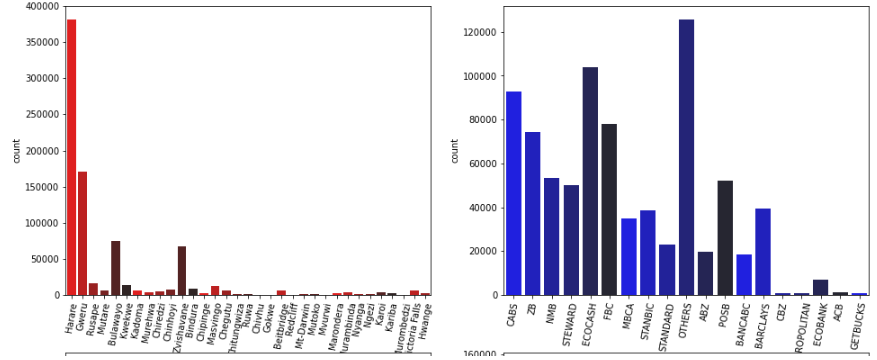
\includegraphics[width=1\linewidth]{image1}
    \caption{Data distribution 1}
    \label{fig:example}
\end{figure}
\newpage
\subsubsection{Box and Whisker Plot}
\begin{figure}[h]
    \centering
    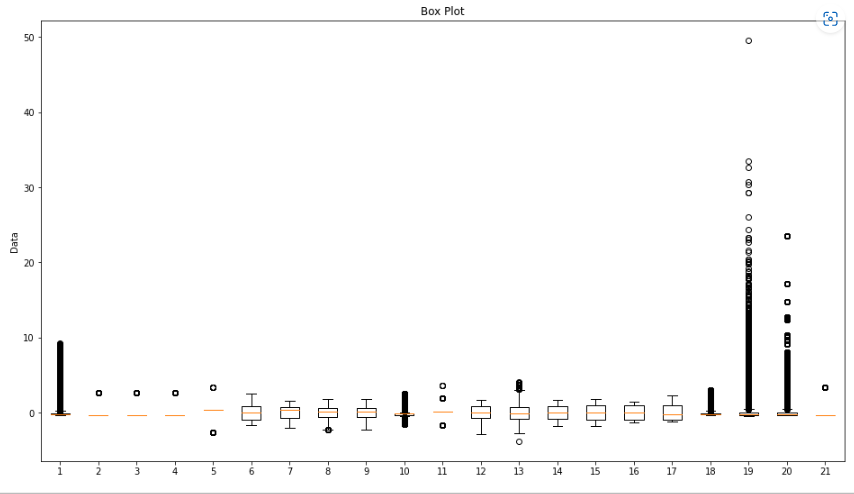
\includegraphics[width=1\linewidth]{image7}
    \caption{Box and Whisker Plot}
    \label{fig:example}
\end{figure}

\subsection{Outliers detections}
The author used the box and whisker plot to determine if there are any outliers in the data set and found out that there
were various columns with many outliers. as shown on the fig below.\\
1) orange - Fraud   2) blue - Not Fraud\\\\
\textbf{data with many otliers\\}
\begin{figure}[h]
    \centering
    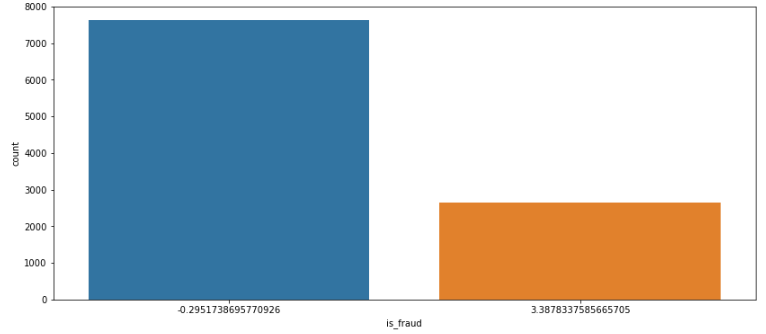
\includegraphics[width=0.7\linewidth]{image5}
    \caption{Data distribution for Outliers}
    \label{fig:example}
\end{figure}
\newpage
The author then carried out EDA to replace outliers with the average values per each column.\\\\
\textbf{data with less otliers\\}
\begin{figure}[h]
    \centering
    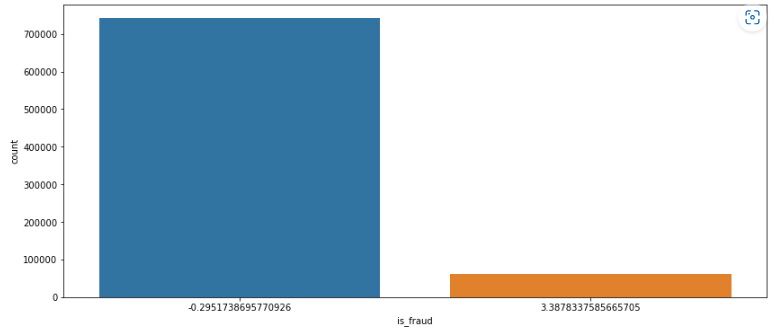
\includegraphics[width=0.7\linewidth]{image6}
    \caption{Data distribution with handled outliers}
    \label{fig:example}
\end{figure}
\subsection{Sampling}
As the researcher was dealing with a huge volume of data set of 1 200 000 rows of transactions it was necessary to 
improve the computational speed of the laptop thus data had to be sampled. The author sampled the data using the 
is\_fraud column and got the uniformly destributed data as shown below.\\
\begin{figure}[h]
    \centering
    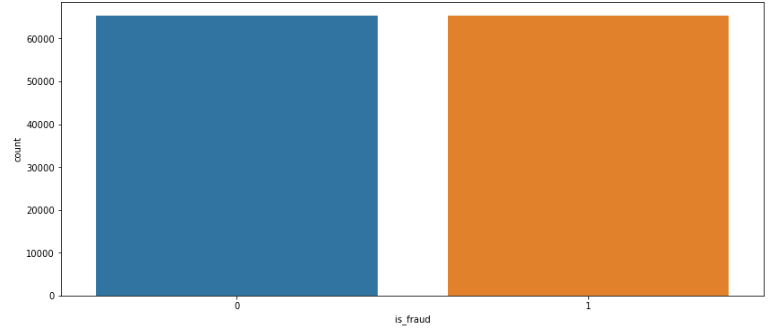
\includegraphics[width=1\linewidth]{image8}
    \caption{Uniformarly distributed data}
    \label{fig:example}
\end{figure}

\subsection{Multivariate analysis for the whole data}
\subsubsection{Correlation Diagram}
this showed that there is very weak relationship between the variables ranging from as little as from 
-0.63 to 0.0016 to 0.82\\ \\
\begin{figure}[h]
    \centering
    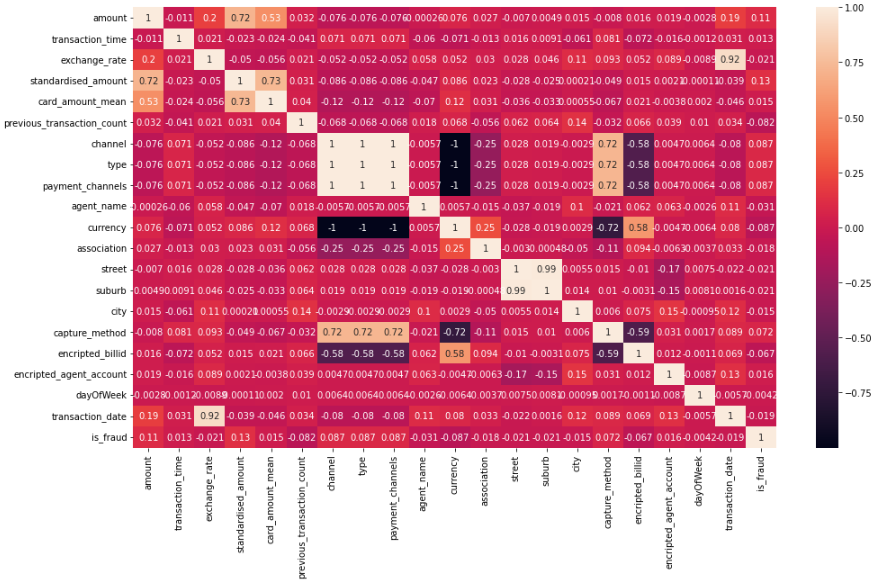
\includegraphics[width=1\linewidth]{image3}
    \caption{Correlation Graph}
    \label{fig:example}
\end{figure}
\subsubsection{Manova Table}
An F-value of -2760 is not possible and likely indicates an error in calculation or data entry.
thus further analysis had to be taken.\\
\begin{figure}[h]
    \centering
    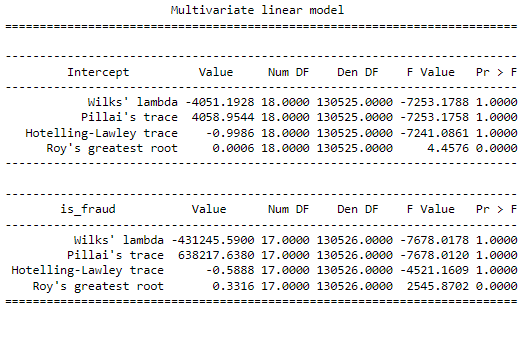
\includegraphics[width=1\linewidth]{image9}
    \caption{Manova Table}
    \label{fig:example}
\end{figure}

\section{Feature Selection and Engineering}

The author performed feature selection and engineering to identify the most relevant variables for the risk modeling 
task. Using the techniques mentioned in the methodology, assessing the correlation between variables to detect 
multicollinearity. Additionally also, used PCA to reduce the number of variables in the 
dataset while preserving the most informative features.

\subsection{Multicollinearity test}
for multicollinearity test the author used VIF.
\newpage 
\begin{table}[h]
    \centering
    \begin{tabular}{|l|l|}
      \hline
      variable & VIF \\ \hline
      amount &   2.620211\\ \hline
             transaction\_time &  24.034300\\ \hline
              exchange\_rate  & 18.169662\\ \hline
                        standardised\_amount  &  4.874732\\ \hline
             card\_amount\_mean  &  3.946724\\ \hline
   previous\_transaction\_count &   1.160809\\ \hline
                      channel    &     inf\\ \hline
                         type    &     inf\\ \hline
             payment\_channels     &    inf\\ \hline
                  agent\_name   & 3.659335\\ \hline
                   currency  & 61.099256\\ \hline
                 association  &  5.780524\\ \hline
                     street & 227.033678\\ \hline
                     suburb & 212.240119\\ \hline
                        city  &  4.013843\\ \hline
             capture\_method &  10.917950\\ \hline
           encripted\_billid  &  6.587185\\ \hline
     encripted\_agent\_account  &  4.465704\\ \hline
                   dayOfWeek  &  2.884910\\ \hline
            transaction\_date &  61.289448\\ \hline
    \end{tabular}
    \caption{Multicollinearity (VIF) table 1}
    \label{Multicollinearity (VIF) table 1}
  \end{table}
\subsubsection{Dropping varibles with range VIF greater than 10}

\newpage
\begin{table}[h]
    \centering
    \begin{tabular}{|l|l|}
        \hline
        variable & VIF \\ \hline
        transaction\_time & 11.176353\\ \hline
        standardised\_amount &  3.612614\\ \hline
        card\_amount\_mean &  3.915085\\ \hline
        previous\_transaction\_count  & 1.153174\\ \hline
        payment\_channels  & 1.964121\\ \hline
        agent\_name  & 3.335068\\ \hline
        association &  4.943633\\ \hline
        city  & 3.785845\\ \hline
        encripted\_billid &  5.154255\\ \hline
        encripted\_agent\_account &  4.000727\\ \hline
        dayOfWeek  & 2.771355\\ \hline
    \end{tabular}
    \caption{Multicollinearity (VIF) table 2}
    \label{Multicollinearity (VIF) table 2}
\end{table}

\subsection{Feature selection}
\vspace{1cm}
\begin{table}[h]
    \centering
    \begin{tabular}{|l|l|}
        \hline
        \textbf{Pearson Feature selection} & \textbf{Chi-Square Feature selection} \\ \hline
        city & city\\ \hline
        card amount mean &  encripted agent account\\ \hline
        association &  association\\ \hline
        agent name  & agent name\\ \hline
        encripted billid  & encripted billid\\ \hline
        payment channels  & payment channels\\ \hline
        standadised amount &  standadised amount\\ \hline
        previous transactions count  & previous transactions count\\ \hline
    \end{tabular}
    \caption{Feature selection table}
    \label{Feature selection table}
\end{table}
\subsection{Selected Features}
\subsubsection{Corelation between features}
\newpage
\begin{figure}[h]
    \centering
    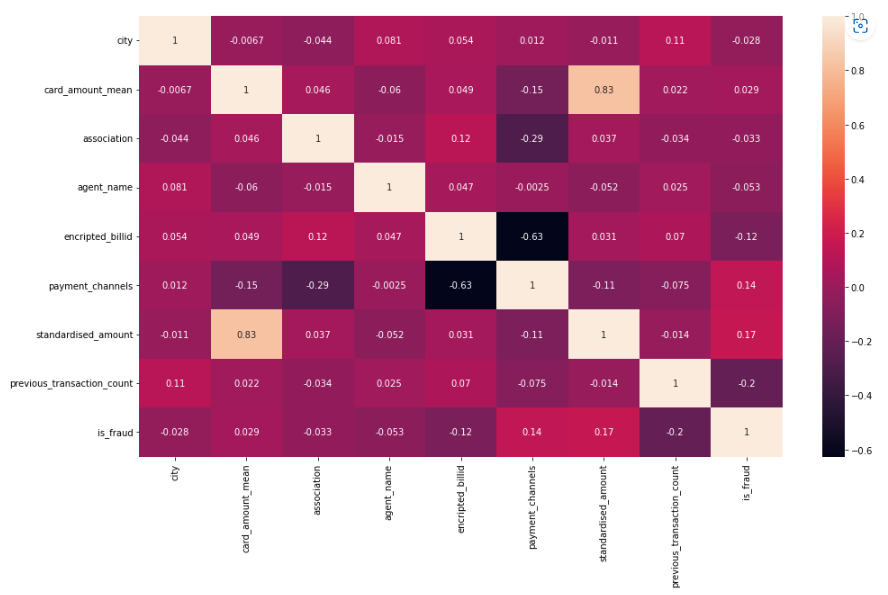
\includegraphics[width=0.9\linewidth]{image13}
    \caption{Selected Features}
    \label{fig:Selected Features}
\end{figure}
\subsubsection{Multivariate analysis between selected Features}
\vspace{1cm}
\begin{figure}[h]
    \centering
    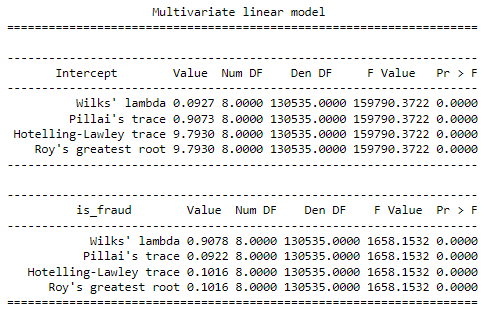
\includegraphics[width=0.7\linewidth]{image14}
    \caption{Multivariate analysis between selected Features}
    \label{fig:Multivariate analysis between selected Features}
\end{figure}
\newpage
\section{Model Training and Evaluation}
After preprocessing the data, the author moved on to training and evaluating the machine learning models.
The author employed K-Nearest Neighbors (KNN), Guasian NB, SVM, Logistic 
Regression, and XGBoost models.\\\\
For each model the dataset was split into training and testing sets using a stratified sampling approach using (70\% to 30\% ).

\subsection{Logistic Regression Model}
\vspace{1cm}
\begin{figure}[h]
    \centering
    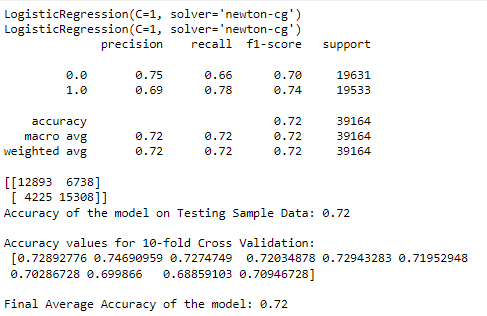
\includegraphics[width=0.8\linewidth]{image15}
    \caption{Logistic Regression Model}
    \label{fig:Logistic Regression Model}
\end{figure}
\newpage
\subsection{XG Boost Model}
\vspace{1cm}
\begin{figure}[h]
    \centering
    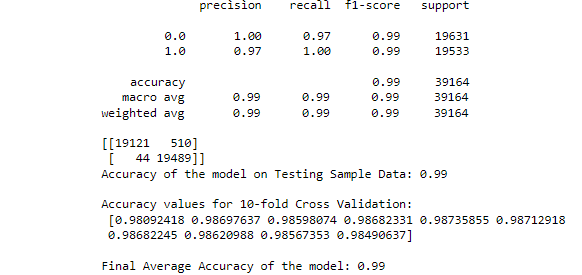
\includegraphics[width=0.8\linewidth]{image16}
    \caption{XG Boost Model}
    \label{fig:XG Boost Model}
\end{figure}
\subsection{K-nearest neighbors Model}
\vspace{1cm}
\begin{figure}[h]
    \centering
    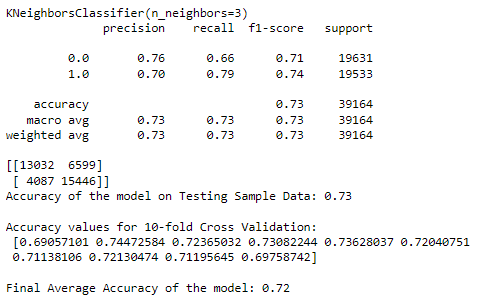
\includegraphics[width=0.8\linewidth]{image17}
    \caption{K-nearest neighbors Model}
    \label{fig:K-nearest neighbors Model}
\end{figure}
\newpage
\subsection{Guasian Naive Bayes Model}
\vspace{0.5cm}
\begin{figure}[h]
    \centering
    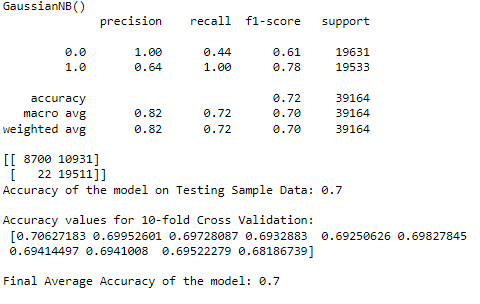
\includegraphics[width=0.6\linewidth]{image18}
    \caption{Guasian Naive Bayes Model}
    \label{fig:Guasian Naive Bayes Model}
\end{figure}
\subsection{Support Vector Model (SVM)}
\vspace{0.5cm}
\begin{figure}[h]
    \centering
    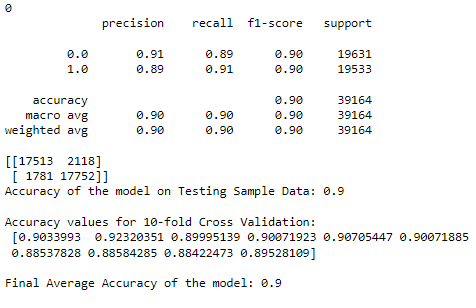
\includegraphics[width=0.6\linewidth]{image19}
    \caption{Support Vector Model (SVM)}
    \label{fig:Support Vector Model (SVM)}
\end{figure}
\section{Model Selection}
Based on results, the author performed model selection to identify the most 
suitable model for detecting fraudulent transactions in the banking sector, considered factors such as model 
performance, interpretability, and computational efficiency. Through this process, the author selected the best-performing 
model that demonstrated a balance between accuracy and computational feasibility.

\newpage
\subsection{Receiver Operating Characteristic (ROC)}
Plotting the TPR against the FPR at various discrimination thresholds. 
The TPR is the fraction of positive instances that are correctly classified, and the FPR is the fraction of 
negative instances that are incorrectly classified.

\subsubsection{For the sampled Dataset}

\begin{figure}[h]
    \centering
    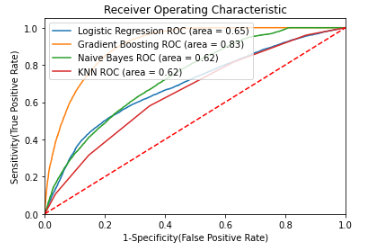
\includegraphics[width=0.7\linewidth]{image21}
    \caption{The ROC}
    \label{fig:The ROC}
\end{figure}

\subsection{Accuracy recall graphs}

\begin{figure}[h]
    \centering
    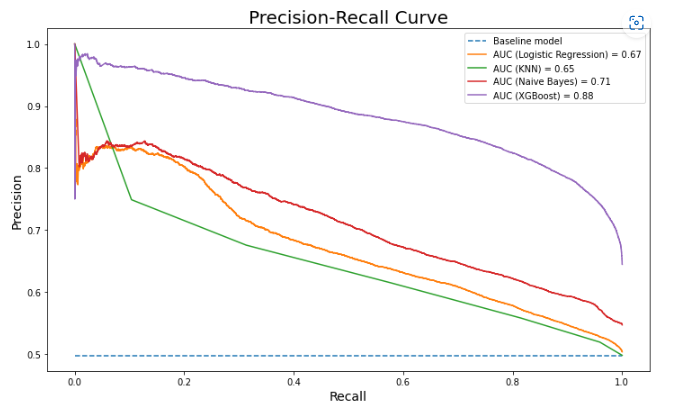
\includegraphics[width=0.7\linewidth]{image22}
    \caption{Accuracy recall graphs}
    \label{fig:Accuracy recall graphs}
\end{figure}

\section{Real-Time Predictions}
In addition to model selection, Author also implemented app for real-time predictions utilising Flask, Jupyter and 
react.js as the backend technologies to expose the machine learning models as RESTful API endpoints. This 
allowed for processing incoming transaction data in real-time and generate predictions efficiently.\\ 

\begin{figure}[h]
    \centering
    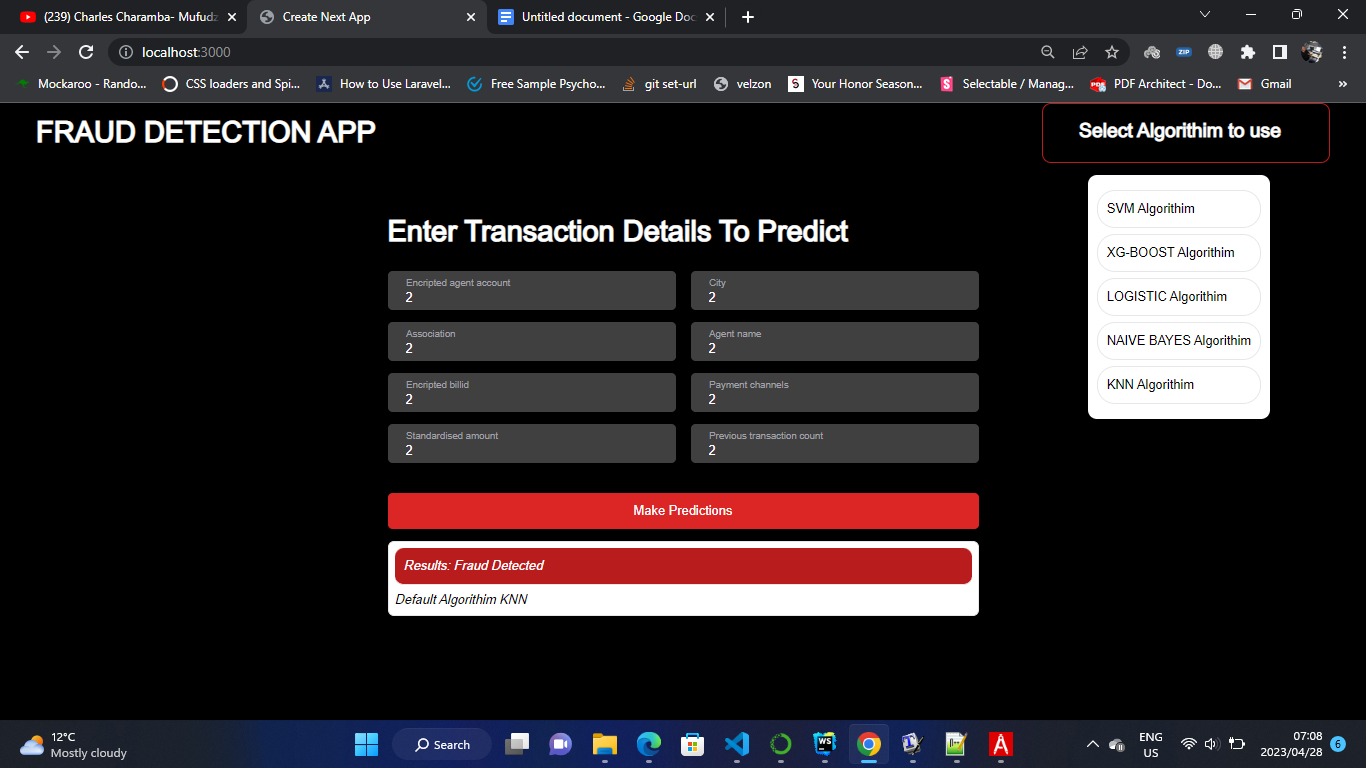
\includegraphics[width=1\linewidth]{image23}
    \caption{Web based application Interface for Real-Time Predictions}
    \label{fig:Web based application Interface for Real-Time Predictions}
\end{figure}

\section{Results and Findings}
The author presented the results and findings derived from the analysis showing performance metrics 
of each model, highlighting their accuracies, precisions, recalls, and F1 scores. Additionally, the author analyzed the 
significance of the selected features and their impact on fraud detection. The author also provided insights into the 
characteristics of fraudulent transactions identified by the models.\\\\
The best perfoming Algorithim was Support vector machine learning algorithim which had an accuracy of 90\% comparing others which were around 70\%
thus this research is in sync with the existing literature which supported SVM as the best algorithim for classification purposes.

\section{Limitations and Future Work}
The author acknowledged the limitations of his study, such as the availability of labeled data, potential biases in the 
dataset, and the scope of the models utilized. Also, the need for further research to enhance the accuracy 
and robustness of the risk modeling approach. Future work could involve incorporating additional features, 
exploring ensemble methods, or considering advanced techniques like deep learning for improved fraud detection.\\\\
In summary, this chapter presented the comprehensive analysis of the data and the results obtained from applying the 
risk modeling techniques outlined in the methodology. It provided insights into the model performance, feature 
importance, and the potential of real-time predictions. The findings contribute to the understanding and advancement 
of fraud detection in the banking sector while acknowledging the scope for further improvements and future research.

\section{Developed App and source code}

\textbf{For the data analysis code visit} \\
https://github.com/C-Maringe/my-thesis/tree/big-data-analysis \\\\
\textbf{For the Fast Api backend code visit} \\
https://github.com/C-Maringe/my-thesis-backend \\\\
\textbf{For the React.js Code visit} \\
https://github.com/C-Maringe/my-thesis \\\\
\textbf{For Real Time Predictions visit} \\
https://my-thesis-sigma.vercel.app \\\\
\chapter{Discussions, Conclusions and Recommendations}

\section{Discussions and Conclusions}

The aim of my undergraduate thesis was to develop a risk modeling approach using big data analytics to detect 
fraudulent transactions in the banking sector. Through the study, I collected a vast amount of transactional data 
from different sources, including customer transaction history, socio-demographic information, and other relevant 
variables that could help identify potential fraudulent transactions.\\\\
After conducting the research, the study concluded that risk modeling with big data is an effective approach to 
detecting fraudulent transactions in the banking sector. By utilizing advanced analytical techniques such as 
machine learning algorithms, the study was able to identify patterns and anomalies in transaction data that may 
indicate fraudulent behavior.\\\\
However, it is important to note that there may be limitations and challenges associated with big data analytics, 
such as data quality issues, privacy concerns, and model interpretability. As such, further research is needed to 
refine the risk modeling approach, address identified limitations, and improve the overall effectiveness of the 
approach.\\\\
The study has practical implications for the banking sector, as it can help institutions improve their fraud 
detection capabilities, reduce the risk of financial losses, and enhance their customer service. By identifying 
fraudulent transactions promptly, banks can take immediate action to protect their customers and maintain the 
integrity of their operations.\\\\
In addition to the conclusions mentioned earlier, the study also found that the use of big data analytics in the 
banking sector can provide several advantages over traditional methods of fraud detection. For example, big data 
analytics can analyze large volumes of transactional data in real-time, enabling banks to detect and respond to 
fraudulent activities more quickly and effectively.\\\\
Moreover, the study revealed that machine learning algorithms can be used to build predictive models that can 
accurately identify potential fraudulent transactions based on various features such as transaction frequency, 
amount, location, and time of day. These predictive models can be trained using historical data to continually 
improve the accuracy of fraud detection over time.\\\\
However, the study also highlighted that there are some challenges associated with implementing a risk modeling 
approach using big data analytics. For example, there may be issues with data quality and consistency that can 
affect the accuracy of the predictive models. Furthermore, the complexity of the algorithms used for risk modeling 
can make it difficult to interpret and understand the results, which may pose challenges for banks in terms of 
regulatory compliance.\\\\
Therefore, the study recommended that banks invest in technologies that can help to improve data quality, such as 
data cleansing and standardization tools. Furthermore, banks should also develop processes to ensure the 
interpretability and transparency of their risk modeling algorithms to comply with regulatory requirements.\\\\
In conclusion, the study has demonstrated that risk modeling with big data analytics is an effective approach to 
detecting fraudulent transactions in the banking sector. By utilizing advanced analytical techniques and predictive 
models, banks can identify fraudulent behavior accurately and more efficiently than traditional methods. However, 
to maximize the effectiveness of this approach, banks must address the challenges associated with data quality, 
algorithm complexity, and interpretability to ensure that the results are accurate, transparent, and compliant 
with regulatory requirements.

\section{Recommendations to the Banking Companies and law makers}

Recommendations for Banking Companies:

\begin{enumerate}
\item Implement risk modeling with big data analytics: Banks should adopt risk modeling with big data analytics as 
a core approach to detecting fraudulent transactions. By using advanced analytical techniques, banks can detect 
fraudulent behavior quickly and efficiently, reducing the risk of financial loss and protecting their customers.
\item Invest in data quality improvement: To maximize the effectiveness of risk modeling, banks must ensure that 
their data is of high quality, consistent, and reliable. Investing in data quality improvement tools such as data 
cleansing and standardization can help improve the accuracy of predictive models and reduce false positives.
\item Develop processes for algorithm interpretability: Banks must develop processes for algorithm interpretability 
to comply with regulatory requirements. This can be achieved by developing models that are transparent and 
explainable, and by providing clear and concise reports on the results of the models.
\end{enumerate}

Recommendations for Lawmakers:

\begin{enumerate}
    \item Promote big data's use in analytics in the financial institutes as banks etc: Lawmakers should encourage 
    the adoption of big data analytics in the banking sector to help detect and prevent fraudulent transactions. 
    This can be achieved by offering incentives such as tax breaks or grants to banks that invest in this 
    technology.
    \item Develop regulations to protect customer privacy: Lawmakers should develop regulations to protect customer 
    privacy and ensure that the use of big data analytics does not compromise the security of sensitive customer 
    data.
    \item Promote algorithmic transparency: Lawmakers should promote algorithmic transparency to ensure that the 
    results of risk modeling are accurate, transparent, and fair. This can be achieved by requiring banks to provide 
    clear and concise reports on the results of their models, and by encouraging them to develop models that are 
    transparent and explainable.\\
\end{enumerate}
In conclusion, the recommendations provided for banking companies and lawmakers can help promote the effective use 
of risk modeling with big data analytics to detect fraudulent transactions in the banking sector. By adopting these 
recommendations, banks can improve their fraud detection capabilities, reduce the risk of financial loss, and 
enhance their customer service. Likewise, lawmakers can help promote the adoption of this technology while 
protecting customer privacy and promoting algorithmic transparency.

 %------------------------------------------------------------------------
%\bibliographystyle{apalike}
%\bibliographystyle{agsm}
%\bibliography{Biblio}

%\chapter{Biblibliography}
\begin{thebibliography}{30}

\bibitem{Gandomi} Gandomi, A., Haider, M., \& Chang, V. (2015). Beyond the hype: \textit{Big data concepts, methods, and applications in healthcare}. Healthcare, 3(3), 124–148. https://doi.org/10.3390/healthcare3030124
\bibitem{Luo} Luo, W. (2017). Big data analytics in financial risk management: \textit{A review}. Journal of Risk Management in Financial Institutions, 11(1), 1–16. https://doi.org/10.1108/JRMFI-04-2016-0014
\bibitem{Li} Li, Y., \& Liao, J. (2018). Big data analytics for financial risk management: \textit{A review}. Expert Systems with Applications, 116, 114–124. https://doi.org/10.1016/j.eswa.2018.04.043
\bibitem{Chen} Chen, H., Chiang, R. H. L., \& Storey, V. C. (2016). Business intelligence and analytics: \textit{From big data to big insights}. MIS Quarterly, 40(2), 1165–1188. https://doi.org/10.25304/misq.2016.40.2.1165
\bibitem{Boudoukh} Boudoukh, J., Richardson, M., \& Whitelaw, R. F. (2007). The future of financial markets: \textit{A new framework for risk management}. Oxford University Press.

\bibitem{Hasnat} Hasnat, M. (2018). Big data analytics: \textit{Current trends and challenges}. Journal of Big Data, 5(1), 1. https://doi.org/10.1186/s40537-017-0117-1.
\bibitem{Sagiroglu} Sagiroglu, S., \& Sinanc, D. (2013). Big data: \textit{A review}. In 2013 international conference on innovations in information technology (pp. 457-460). Atlantis Press. https://doi.org/10.2991/itiit.2013.31.
\bibitem{Srivastava} Srivastava, J., \& Gopalkrishnan, V. (2015). Big data analytics: \textit{A survey}. ACM Computing Surveys (CSUR), 48(3), 1-43. https://doi.org/10.1145/2765469
\bibitem{Lackovic} Lackovic, D., Ilic, M., \& Stanojevic, M. (2016). Big data challenges and trends. In 2016 IEEE 38th international conference on soft computing and intelligent systems (pp. 150-155). IEEE. https://doi.org/10.1109/sicais.2016.7509727.
\bibitem{Jurafsky} Jurafsky, D., \& Martin, J. H. (2008). Speech and language processing (2nd ed.). \textit{Prentice Hall}.
\bibitem{Cleveland} Cleveland, W. S. (1993). Visualizing data. \textit{Hobart Press}.
\bibitem{McAfee} McAfee, A., \& Brynjolfsson, E. (2012). Big data: The management revolution. \textit{Harvard Business Review Press}.
\bibitem{Khrestina} Khrestina, K., Shevchenko, A., \& Yakovlev, A. (2017). Machine learning for fraud detection and risk management in financial services. \textit{In Proceedings of the 2017 ACM SIGKDD Conference on Knowledge Discovery and Data Mining (KDD '17) (pp. 1555-1564). ACM}.
\bibitem{Villalobos} Villalobos, J. A., \& Silva, A. (2017). A machine learning approach to money laundering detection. \textit{Expert Systems with Applications, 82, 386-395}.
\bibitem{Zareapoor} Zareapoor, M., \& Shamsolmoali, S. M. (2015). A comparative study of machine learning algorithms for credit card fraud detection. \textit{Journal of Information Security, 6(2), 1-12}.
\bibitem{Pun} Pun, C. S., \& Lawryshyn, A. (2012). A hybrid neural network and rule-based expert system for credit card fraud detection. \textit{Expert Systems with Applications, 39(11), 9725-9733}.



\bibitem{Jagtiani} Jagtiani, J., \& Liao, J. (2018). Big data analytics in the banking sector: \textit{A review}. Expert Systems with Applications, 116, 114–124. https://doi.org/10.1016/j.eswa.2018.04.043
\bibitem{Saunders} Saunders, A., \& Allen, L. (2007). Financial markets and institutions: \textit{A modern perspective}. McGraw-Hill Education.
\bibitem{Dicuonzo} Dicuonzo, F., Nocera, F., \& Perrone, G. (2019). Big data analytics in banking: \textit{A literature review}. Computers \& Industrial Engineering, 132, 106–117. https://doi.org/10.1016/j.cie.2019.02.029
\bibitem{Hossein} Hossein, S., \& Hashemi, S. M. (2018). New approaches to risk management in the banking sector after the 2008 financial crisis. Journal of Risk Finance, 19(3), 213–229. https://doi.org/10.1108/JRF-06-2017-0093
\bibitem{Florio} Florio, G., \& Leoni, G. (2017). The role of risk management in the financial crisis. Journal of Risk Finance, 18(4), 328–340. https://doi.org/10.1108/JRF-06-2016-0079



\bibitem{Firebase} Firebase.(2021) Docs (Online). Available at: https://firebase.google.com/docs/hosting (Accessed 28 July 2021)

\end{thebibliography}   % For Gather Purpose Only
%\setlinespacing{1.44}
%\bibliographystyle{amsplain}
%-------------------------------------------------------------------------
%\typeout{Appendix}
\appendix
\chapter{Resources}

\textbf{For the data analysis code visit} \\
https://github.com/C-Maringe/my-thesis/tree/big-data-analysis \\\\
\textbf{For the Fast Api backend code visit} \\
https://github.com/C-Maringe/my-thesis-backend \\\\
\textbf{For the React.js Code visit} \\
https://github.com/C-Maringe/my-thesis \\\\
\textbf{For Real Time Predictions visit} \\
https://my-thesis-sigma.vercel.app \\\\



%-------------------------------------------------------------------------
\end{document}
% ------------------------------------------------------------------------
